\chapter{System Analysis and Design}

The development of a complex calendar management system like Jadwal requires careful analysis of requirements and thoughtful system design to ensure robust functionality and seamless user experience. This chapter presents a detailed examination of Jadwal's architecture, from its core requirements to the intricate relationships between system components. Through use case diagrams, activity diagrams, class diagrams, and database design (both ER and Relational), we provide a comprehensive blueprint of how Jadwal transforms its innovative concepts into a practical, functioning system.

\section{Introduction}

A well-designed system requires a good understanding of both functional and non-functional requirements to meet user expectations and deliver a seamless experience.

This section shows the functional and non-functional requirements which is the backbone of Jadwal's development. The functional requirements focus on core features, such as user authentication, calendar integration and event management. Ensuring the users can effectively manage their schedules. The non-functional requirements focuses on performance, security, compatibility, and user experience, ensuring the application stands well with the industry standards by providing efficient interface.

Combining all these requirements helps in the design and implementation of Jadwal which will lead to a better application solving real issues and meeting the needs of the user.

\section{Functional Requirements}

The following requirements outline the core features and capabilities that Jadwal must provide to fulfill its purpose as an intelligent calendar management system:
\begin{itemize}
    \item The user shall be able to access their account using either Google OAuth or magic link via Email. For new users, a new account is created, and for existing users, they are given access to their account directly.
    \item The system shall send a welcome email to new users.
    \item The user should be able to create a calendar.
    \item The user should be able to connect a calendar using CalDAV.
    \item The user should be able to connect their WhatsApp account.
    \item The user should be able to add events manually.
    \item The user should be able to view integrated calendar.
    \item The user should be able to schedule prayer times.
    \item The system shall send event notifications to the user.
    \item The system shall add the WhatsApp extracted events to the calendar. If a conflict occurs, the user shall get a notification to resolve the conflict with suggestions.
    \item The user should be able to manage scheduling conflicts.
\end{itemize}

Each functional requirement listed above will be explained in details through a use case description in the coming sections.

\newpage

\section{Non-Functional Requirements}

While functional requirements define what the system does, non-functional requirements specify how the system performs its functions. These requirements focus on the quality attributes, performance standards, and technical constraints that ensure Jadwal delivers a reliable, secure, and user-friendly experience.

\begin{itemize}
    \item \textbf{Platform Compatibility:} The app shall be compatible with iOS devices running iOS 16.0 or later.
    \item \textbf{Performance:} The app shall load the main calendar view within 3 seconds on 5G with speeds above 200mpbs.
    \item \textbf{User Experience:} The user interface shall follow iOS Human Interface Guidelines for consistency and ease of use.
    \item \textbf{Security:} All data transmissions between the app and servers shall be encrypted using HTTPS.
\end{itemize}


\section{Security Architecture}

In today's digital world, security is a key concern for any application that handles user data. Jadwal places a strong emphasis on ensuring the security and trustworthiness of the platform for its users, implementing multiple layers of security measures to protect user data.

\subsection{Authentication: Magic Token and JWT Tokens}

To provide secure authentication, Jadwal implements Magic Token authentication. Instead of relying on traditional username and password combinations, which is vulnerable to various attacks, such as credentials leakage through database dumps. To mitigate this, Jadwal sends the users trying to authenticate a secure magic link to their verified email address. A magic link is a special URL that contains a secure token, the magic token. For example:

\begin{verbatim}
    https://jadwal.app/magic-link?token=some-uuid
\end{verbatim}

In this URL, \texttt{some-uuid} is the secure token, which we call magic token, and the complete URL is what we call the magic link. When sent to the user's email, clicking this link proves they have access to the email account they're trying to use.

When a user logs in using the magic link sent to their email, Jadwal secures the user's account by verifying the magic token provided. This ensures that the account can only be accessed by the legitimate user who has access to the registered email account. To enhance security, the magic token has a limited lifetime of 15 minutes, significantly reducing the window of opportunity for potential attacks.

Upon successful magic token verification, Jadwal issues two JWTs (JSON Web Token) signed with the platform's private key. This digital signature serves as a cryptographic guarantee of the token's authenticity, allowing the system to verify that tokens haven't been tampered with and were legitimately issued by Jadwal's own system.

The first JWT is called the \textit{access token}, and it is a short-lived token that expires after 5 minutes. This token is back by the client in the \textit{Authorization} HTTP header as a \textit{\gls{bearer-authentication}} token, also known as \textit{token authentication}, to authenticate themselves when calling protected resources.

The second JWT is called the \textit{refresh token}, and it is transmitted securely encrpyted in-transit to the device. This is a long-lived token that allows the user to ask for a new token every time the \text{access token} expires.

\subsection{Magic Token Storage and Security}

To ensure the security of magic tokens, Jadwal implements secure storage practices for storing the magic token in the database. Magic tokens are never stored in their original form; instead, they are protected using the SHA-256 hashing algorithm before being saved in the database. When verifying magic tokens, the system hashes the user-provided magic token and compares it with the stored hash, ensuring that even in the unlikely event of a database breach, the original magic tokens remain secure.

\subsection{Secure Logout Implementation}

Jadwal implements a secure logout mechanism by removing the refresh token from the user's device upon logout. This practice ensures that once a user logs out, their refresh token cannot be reused for unauthorized access, maintaining the integrity of user sessions.

\subsection{Transparency Through Open Source}

As part of our commitment to security and privacy, Jadwal will be released as open-source software. This transparency allows security experts and users to verify our security implementations and privacy practices. Users can inspect exactly how their data is handled and verify that our privacy commitments are upheld through code review.


\section{System Architecture}

Jadwal implements a modern, distributed architecture leveraging gRPC (Google Remote Procedure Call) for efficient communication between its components. The system is divided into several key services, each responsible for specific functionality while maintaining high performance and reliability.

Jadwal implements a modern architecture leveraging \gls{connectrpc} for communication between the backend and the mobile app for efficient communcation. It also enhances the developer experience and makes the developer think about the design of the API before the programming language to use.

\begin{figure}[!h]
    \centering
    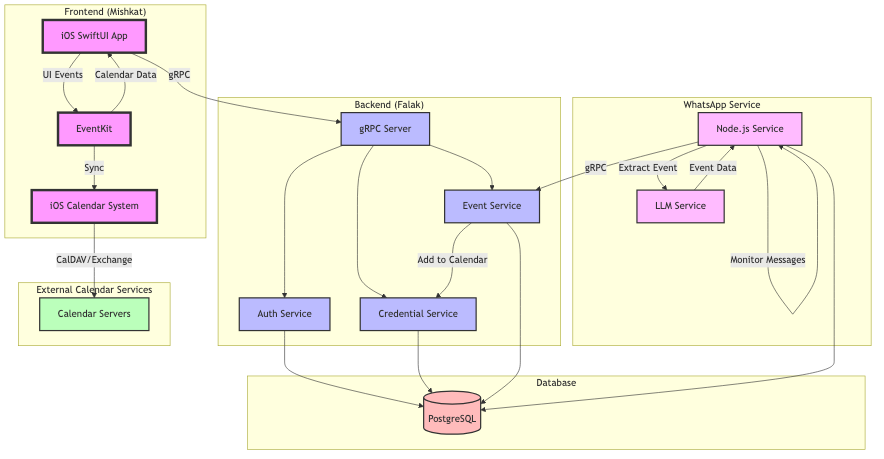
\includegraphics[width=0.6\textwidth]{images/architecture.png}
    \caption{Jadwal System Architecture}
    \label{fig:architecture}
\end{figure}

The architecture, shown in \textbf{Figure~\ref{fig:architecture}}, consists of the following main components:

\begin{enumerate}
    \item \textbf{Frontend (Mishkat)}
          \begin{itemize}
              \item iOS SwiftUI application implementing the client-side \gls{connectrpc} communication
              \item Handles user interface and local state management
          \end{itemize}

    \item \textbf{Backend (Falak)}
          \begin{itemize}
              \item \Gls{connectrpc} server implementing the primary business logic
              \item Auth service managing user authentication
              \item Calendar service making use of a CalDAV client enabling connection to our \Gls{baikal} server to add events to the WhatsApp calendar
              \item Event consumer processing WhatsApp events from the messages queue
              \item Event producer and consumer for extracted calendar events to process
          \end{itemize}

    \item \textbf{Wasapp (WhatsApp) Service}
          \begin{itemize}
              \item \gls{bun} HTTP RESTful API that allows \textit{falak} to communicate with this 
              \item \gls{whatsappwebjs} client for message receiving
              \item Event producer publishing detected events to the message queue
          \end{itemize}

    \item \textbf{\gls{rabbitmq} Queue}
          \begin{itemize}
              \item \gls{rabbitmq} handling asynchronous event processing
              \item Ensures reliable delivery of WhatsApp events to the backend
              \item Ensures reliable handling of adding calendar events and sending user notifications
          \end{itemize}

    \item \textbf{Database}
          \begin{itemize}
              \item \gls{postgresql} storing customer data, calendar credentials, device IDs, magic tokens, Wasapp chats, and Wasapp messages
              \item Maintains data consistency across all services
          \end{itemize}
\end{enumerate}

This architecture enables several key benefits:

\begin{itemize}
    \item \textbf{Performance}: \gls{connectrpc}'s use of \gls{protobuf} and \gls{http2} ensures efficient communication between services
    \item \textbf{Scalability}: Separate services can be scaled independently based on load
    \item \textbf{Reliability}: Message queue ensures no events are lost during processing
    \item \textbf{Maintainability}: Clear separation of concerns makes the system easier to maintain and update
\end{itemize}

\section{System Use Cases}
The functionality of Jadwal can be best understood through its various use cases, which demonstrate how users interact with the system. Each use case details specific interactions and flows that make up the core functionality of Jadwal. The diagram in Figure~\ref{fig:use-case-diagram} provides an overview of all use cases and their relationships.

\textbf{Figure~\ref{fig:use-case-diagram}} shows the complete use case diagram for Jadwal's system, illustrating the relationships between these fourteen distinct use cases and their actors.

\begin{figure}[!h]
    \centering
    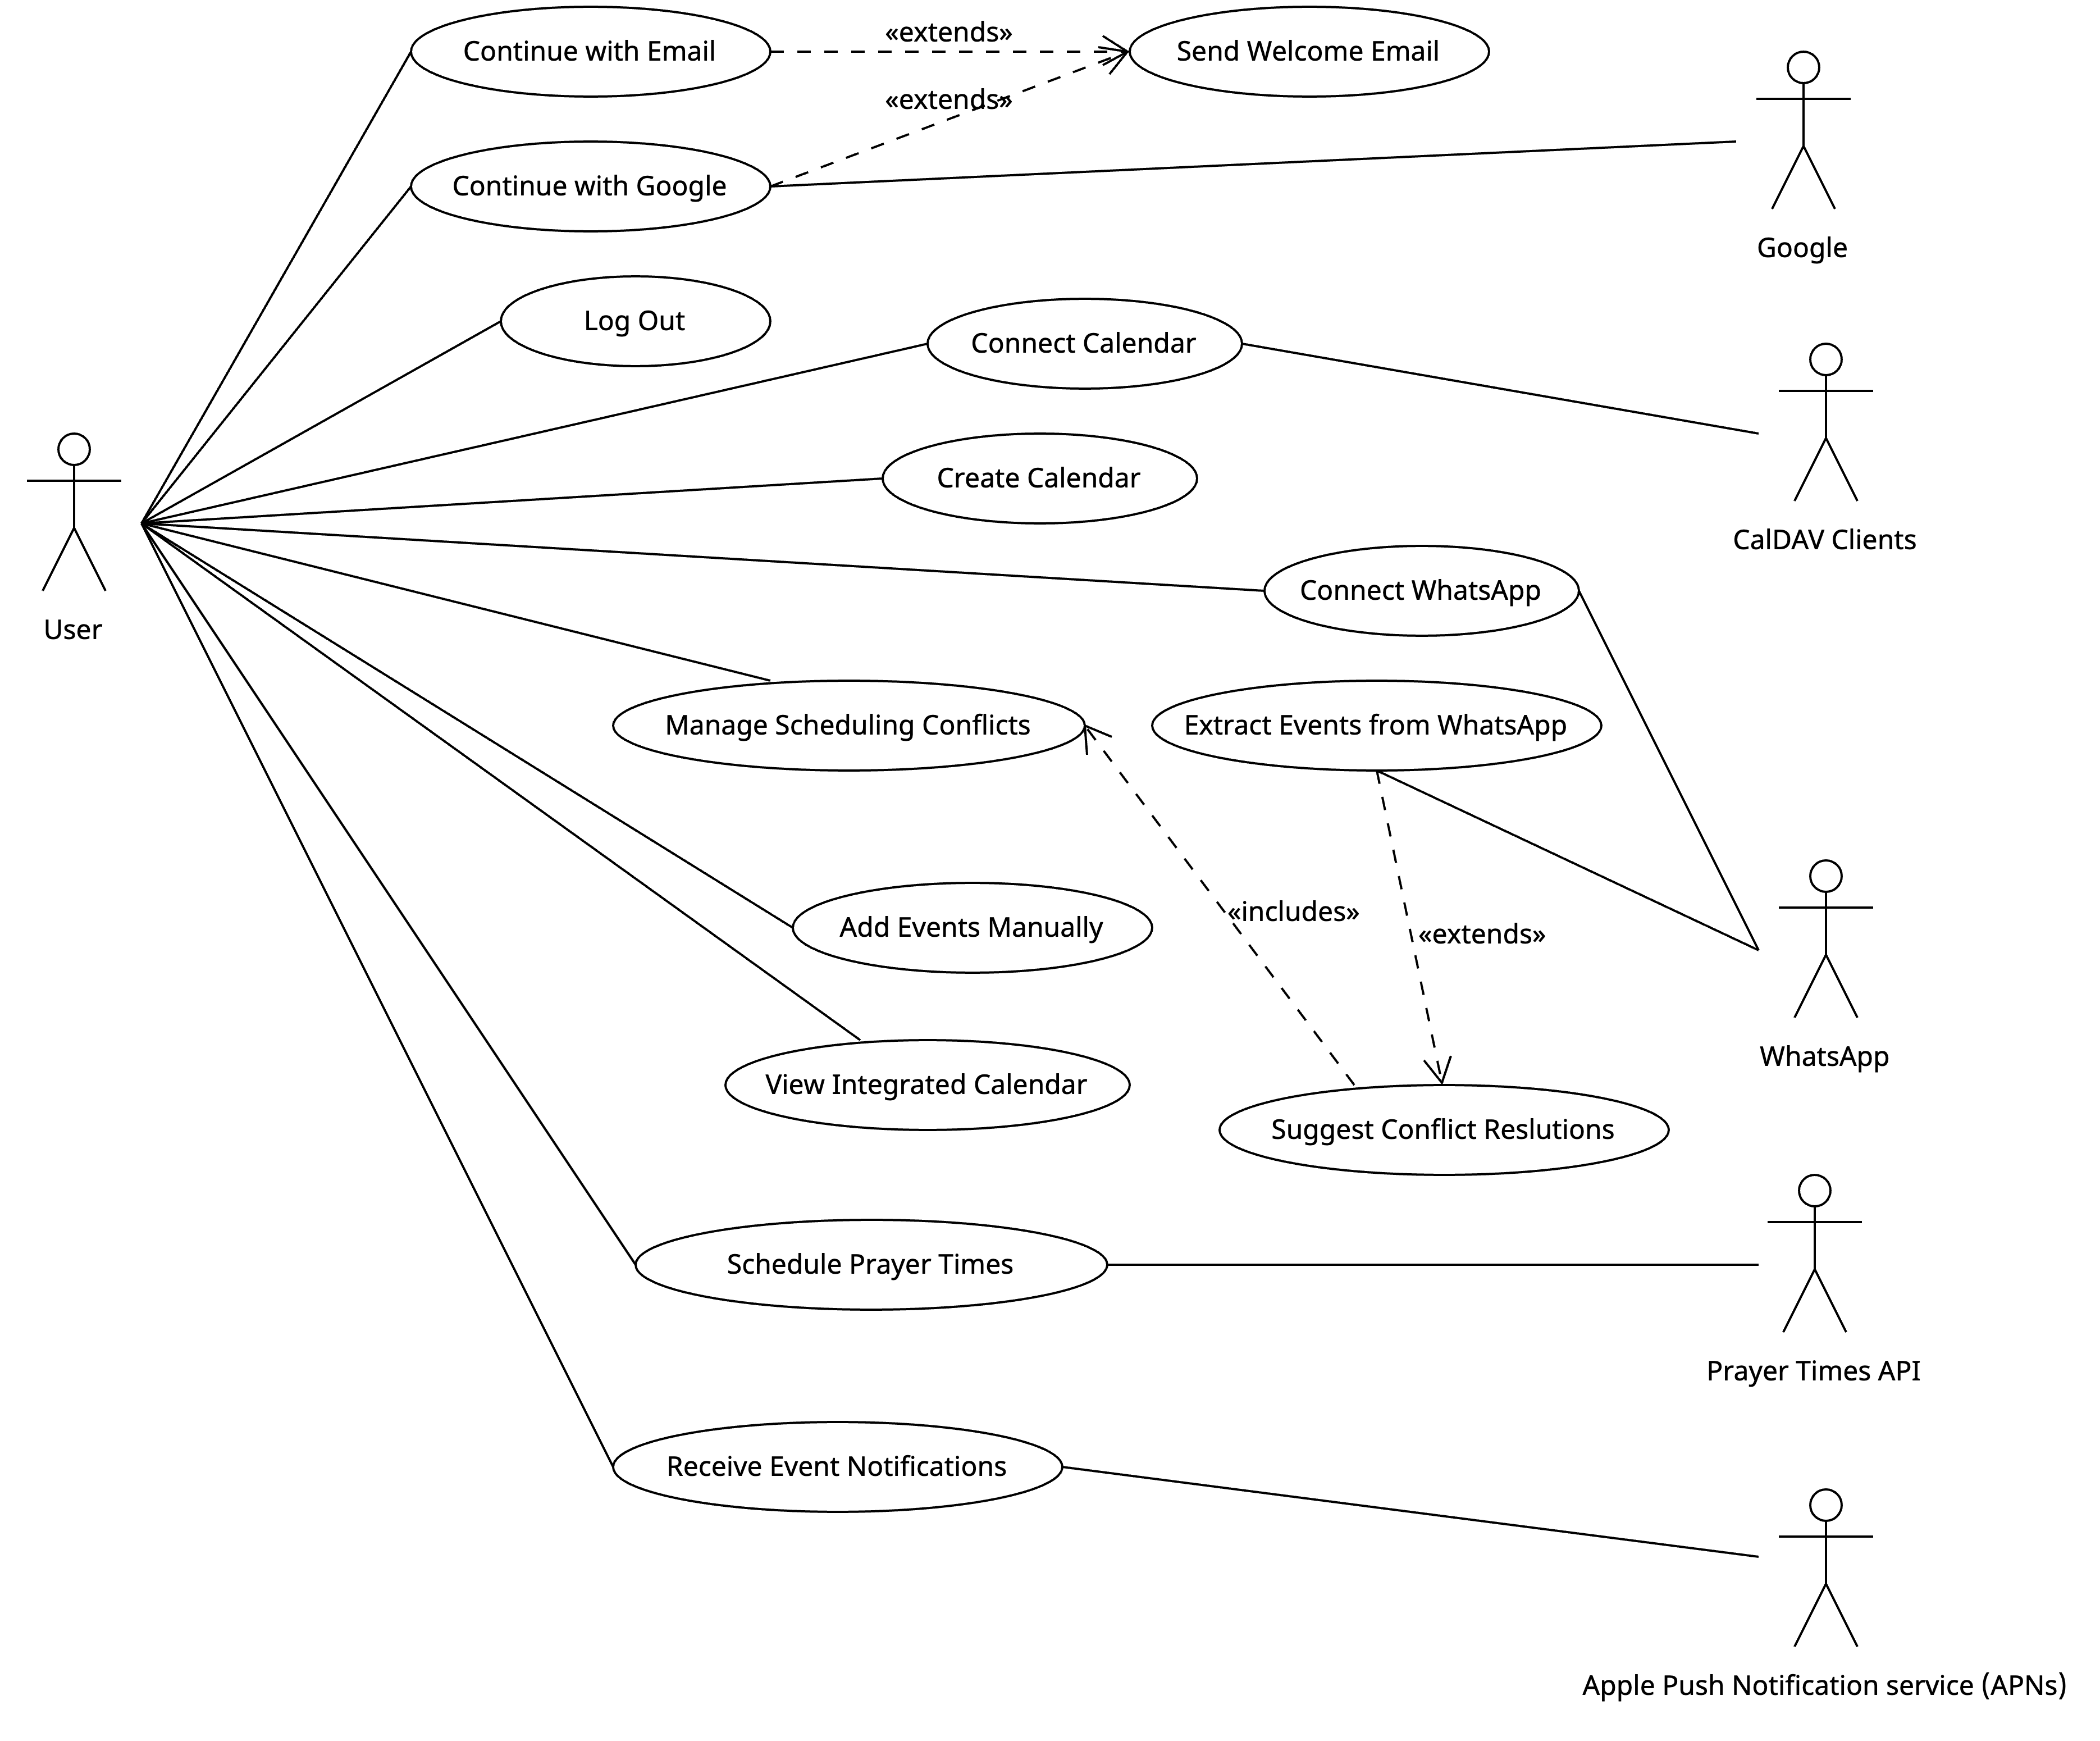
\includegraphics[width=\textwidth]{images/use-case-diagram.png}
    \caption{Use Case Diagram of Jadwal}
    \label{fig:use-case-diagram}
\end{figure}

\subsection{Authentication and User Management}
User authentication is the first interaction point with Jadwal. We support both email-based authentication through magic links and Google OAuth to provide secure and convenient access options. The following use cases detail the login flows and account management features.

\begin{usecase}{Continue with Email}
  \ucbasicinfo{High}{Regular}
  \ucshortdescription{This UC allows users to login or create an account using their email.}
  \uctrigger{This UC starts when the user enters their email to the system.}
  \ucactors{User}{None}
  \ucpreconditions{User must have an email}
  \ucrelationships{Send Welcome Email}{N/A}{N/A}
  \ucinputsoutputs{
    \begin{itemize}
      \item \textbf{Email} (Source: User)
      \item \textbf{Magic Link (from email)} (Source: User)
    \end{itemize}
  }{
    \begin{itemize}
      \item \textbf{Magic link email} (Destination: User)
      \item \textbf{Confirmation messages} (Destination: User Interface)
      \item \textbf{JWT} (Destination: App)
    \end{itemize}
  }
  \ucmainflow{
    \begin{enumerate}
      \item The user enters their email.
            \ucinfo{System displays an email input field.}
      \item System creates an account if the user has no account, and then generates and sends the magic link.
            \ucinfo{App displays ``Check your email'' message.}
      \item The user clicks the magic link in the email.
            \ucinfo{The app is opened on the device of the user.}
      \item The app sends the token to the system to log the user in.
            \ucinfo{System verifies token and logs user in.}
    \end{enumerate}
  }
  \ucalternateflows{
    \begin{itemize}
      \item The user cancels the authentication request.
    \end{itemize}
  }
  \ucexceptions{
    \begin{itemize}
      \item Invalid email format.
      \item Magic link token expired or invalid.
      \item \textbf{Request sending failure}: If sending the request fails due to network issues, the system prompts the user to try again.
    \end{itemize}
  }
  \ucconclusion{This UC ends when the user is logged in.}
  \ucpostconditions{The system generates a JWT.}
  \ucspecialrequirements{An email server must be present to send magic link email.}
\end{usecase}

\begin{figure}[!h]
  \centering
  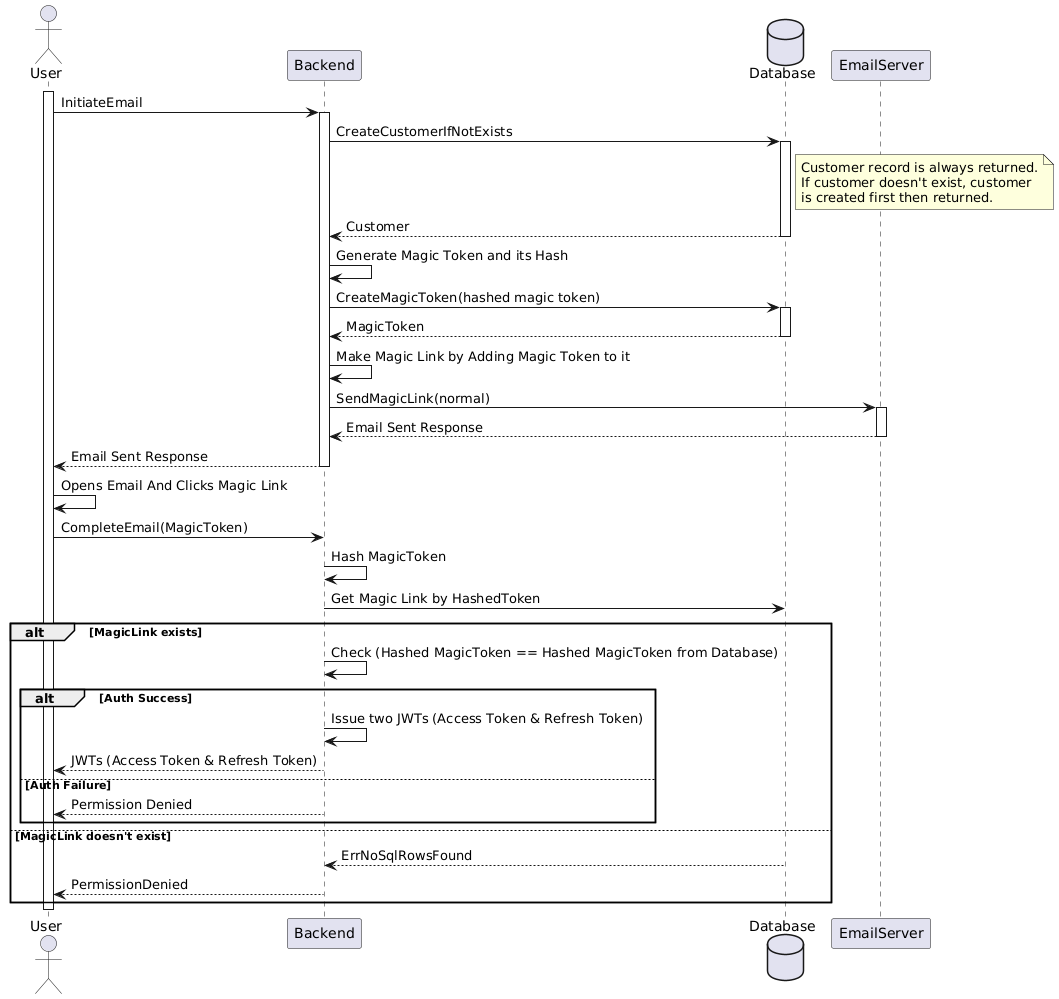
\includegraphics[width=\textwidth]{images/docs/diagrams/sequence-diagrams/all-sequence-diagrams/Continue with Email.png}
  \caption{Continue with Email Sequence Diagram}
  \label{fig:seq/continue-with-email}
\end{figure}

The "Continue with Email Sequence Diagram", shown in \textbf{Figure~\ref{fig:seq/continue-with-email}}, illustrates the process of email-based magic link authentication, involving interactions between the User, Backend, Database, and EmailServer. The process begins when the user initiates an action, such as signing up or logging in. The backend executes the CreateCustomerIfNotExists function to retrieve an existing customer record or create a new one if none exists. Once the customer is identified, the backend generates a magic token and its hashed version using the GenerateMagicToken function. The hashed token is stored in the database, and a magic link containing the token is created. The backend then sends the magic link to the user's email using the SendEmail function via the email server. The user clicks the magic link, triggering the CompleteFlow(MagicToken) request to the backend, where the provided token is validated against the stored hashed token in the database. If the tokens match, authentication succeeds, and the backend issues a JSON Web Token (JWT) to the user for future access. In cases where the token is invalid, expired, or the customer record is missing, the system responds with appropriate errors, such as PermissionDenied or EntryNotFound. This diagram demonstrates a secure flow for handling authentication via email magic links.
\begin{usecase}{Continue with Google}
  \ucbasicinfo{High}{Regular}
  \ucshortdescription{This UC allows users to login or sign up with their Google account.}
  \uctrigger{This UC starts when the user clicks ``Continue with Google'' button in the app.}
  \ucactors{User}{Google}
  \ucpreconditions{The user must have an active Google account.}
  \ucrelationships{Send Welcome Email}{N/A}{N/A}
  \ucinputsoutputs{
    \begin{itemize}
      \item \textbf{Google access token} (Source: User)
    \end{itemize}
  }{
    \begin{itemize}
      \item \textbf{Authentication response} (Destination: User)
      \item \textbf{JWT} (Destination: App)
    \end{itemize}
  }
  \ucmainflow{
    \begin{enumerate}
      \item The user click continue with Google.
        \ucinfo{App uses OAuth to authenticate with Google}
      \item App sends Google access token to the system.
        \ucinfo{System verifies the token is issued for us and then issues JWT for usage within the app.}
    \end{enumerate}
  }
  \ucalternateflows{
    \begin{itemize}
      \item The user cancels the authentication request.
    \end{itemize}
  }
  \ucexceptions{
    \begin{itemize}
      \item Google access token invalid or expired.
      \item \textbf{Request sending failure}: If sending the request fails due to network issues, the system prompts the user to try again.
    \end{itemize}
  }
  \ucconclusion{This UC ends when the user is logged in.}
  \ucpostconditions{The system generates a JWT.}
  \ucspecialrequirements{A google client must be present for the validation of the access token to be possible.}
\end{usecase}

\begin{figure}[!h]
  \centering
  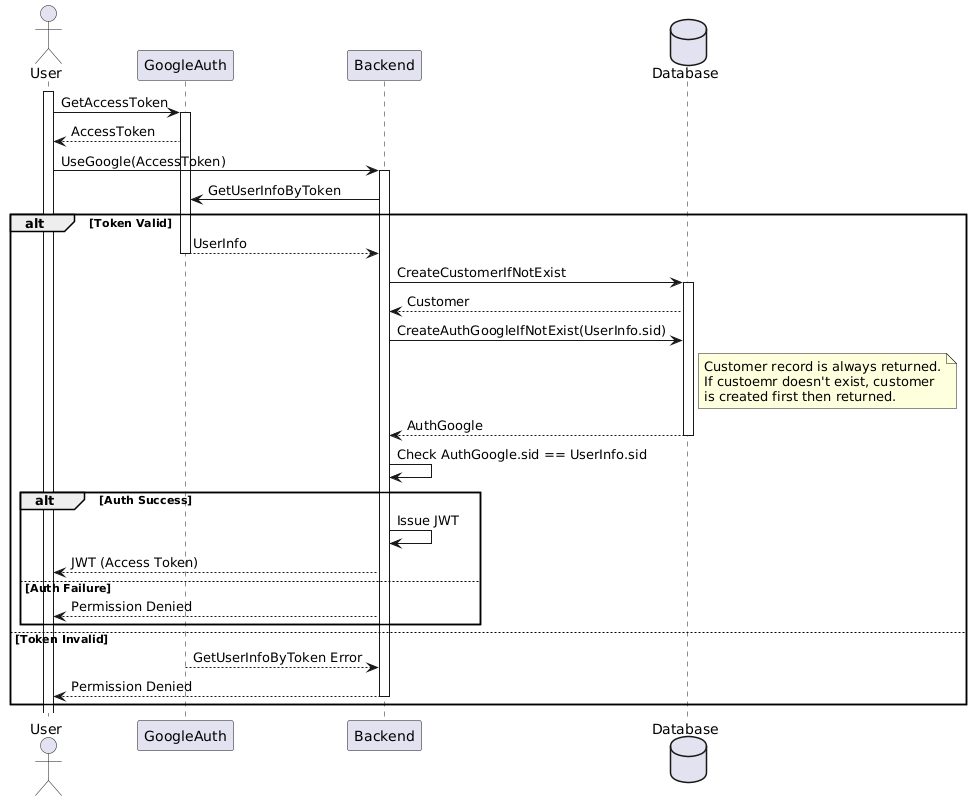
\includegraphics[width=\textwidth]{images/docs/diagrams/sequence-diagrams/all-sequence-diagrams/Continue with Google.png}
  \caption{Continue with Google Sequence Diagram}
  \label{fig:seq/continue-with-google}
\end{figure}
\begin{usecase}{Send Welcome Email}
    \ucbasicinfo{Low}{Regular}
    \ucshortdescription{This UC welcomes the user to the platform.}
    \uctrigger{This UC starts when the user account is created.}
    \ucactors{User}{None}
    \ucpreconditions{User account must be created in the system.}
    \ucrelationships{N/A}{N/A}{N/A}
    \ucinputsoutputs{
      \begin{itemize}
        \item \textbf{User name} (Source: System)
        \item \textbf{Welcome email template} (Source: System)
      \end{itemize}
    }{
      \begin{itemize}
        \item \textbf{Welcome email} (Destination: User)
      \end{itemize}
    }
    \ucmainflow{
      \begin{enumerate}
        \item The system fetches the user information.
          \ucinfo{The database is used.}
        \item The system fetches the send welcome email template.
          \ucinfo{The template is filled with the user name.}
        \item The system sends the email with the template.
          \ucinfo{The email is received by the user welcoming them.}
      \end{enumerate}
    }
    \ucexceptions{
      \begin{itemize}
        \item Email server is down.
      \end{itemize}
    }
    \ucconclusion{This UC ends when the user receives an email from us welcoming them.}
    \ucspecialrequirements{An email server must be present to send welcome email.}
\end{usecase}

\begin{figure}[!h]
  \centering
  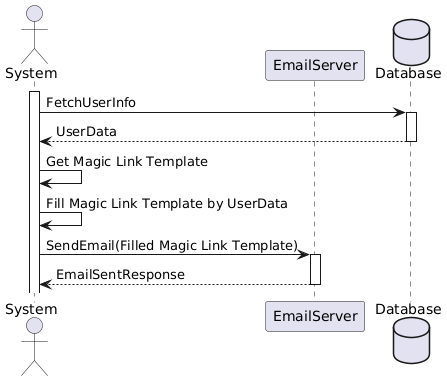
\includegraphics[width=\textwidth]{images/docs/diagrams/sequence-diagrams/all-sequence-diagrams/Send Welcome Email.png}
  \caption{Send Welcome Email Sequence Diagram}
  \label{fig:seq/send-welcome-email}
\end{figure}
\clearpage
\begin{usecase}{Continue with Google}
  \ucbasicinfo{\#2}{HIGH}{Regular}
  \ucshortdescription{This UC allows users to login or continue with Google if we have a Google account}
  \uctrigger{This UC starts when the user enters their email to the system.}
  \ucactors{User}{Google}
  \ucpreconditions{User must have an activated or valid Google email.}
  \ucrelationships{Send Welcome Email}{N/A}{N/A}
  \ucinputsoutputs{
    \begin{itemize}
      \item \textbf{Google account} (Source: User)
      \item \textbf{Authentication request to Google} (Source: System)
    \end{itemize}
  }{
    \begin{itemize}
      \item \textbf{Success or error message} (Destination: User)
      \item \textbf{Authentication response} (Destination: Google)
    \end{itemize}
  }
  \ucmainflow{
    \begin{enumerate}
      \item The user click continue with Google.
        \ucinfo{System displays "continue with Google" button}
      \item Authentication request.
        \ucinfo{A request sent to Google for user authentication and get JWT and sent it to the system, while the system will generate a our JWT}
      \item Authentication response.
        \ucinfo{Confirmation of successful authentication}
    \end{enumerate}
  }
  \ucalternateflows{
    \begin{itemize}
      \item User cancels authentication
      \item Authentication failure
    \end{itemize}
  }
  \ucexceptions{
    \begin{itemize}
      \item Invalid Google email
      \item Network issue
    \end{itemize}
  }
  \ucconclusion{}
  \ucpostconditions{The user is successfully authenticated and redirected to the main application interface}
  \ucbusinessrules{
    \begin{itemize}
      \item User should have valid Google account
    \end{itemize}
  }
  \ucspecialrequirements{Sign-in page should display clear button and error message}
\end{usecase}

\subsection{Calendar Management}
At its core, Jadwal helps users manage their calendars effectively. These use cases show how users can create new calendars, connect existing ones through CalDAV, and view all their calendars in one integrated interface.

\begin{usecase}{Connect Calendar}
    \ucbasicinfo{Medium}{Regular}
    \ucshortdescription{This UC allows the user to access their iOS device calendars through EventKit and configure CalDAV accounts.}
    \uctrigger{This UC is triggered when the user first launches the app or manually initiates calendar access.}
    \ucactors{User}{EventKit}
    \ucpreconditions{User must be logged in}
    \ucrelationships{N/A}{N/A}{N/A}
    \ucinputsoutputs{
        \begin{itemize}
            \item \textbf{Calendar Access Permission} (Source: User)
            \item \textbf{CalDAV Account Credentials} (Source: Backend)
        \end{itemize}
    }{
        \begin{itemize}
            \item \textbf{Local Calendar Access Status} (Destination: System)
            \item \textbf{Calendar Events} (Destination: App)
        \end{itemize}
    }
    \ucmainflow{
        \begin{enumerate}
            \item The system requests calendar access permission from the user.
                  \ucinfo{The app requests EventKit authorization to access device calendars.}
            \item The system retrieves CalDAV account credentials from the backend.
                  \ucinfo{The app fetches encrypted credentials for our CalDAV server.}
            \item The system configures CalDAV accounts through iOS's native calendar system.
                  \ucinfo{EventKit handles direct communication with all CalDAV servers (both ours and external ones).}
            \item The system fetches calendar events using EventKit.
                  \ucinfo{Events are fetched from all configured calendar accounts through iOS's native calendar system.}
            \item The system sets up local notifications for calendar events.
                  \ucinfo{Notifications are scheduled locally based on event reminders.}
        \end{enumerate}
    }
    \ucalternateflows{
        \begin{enumerate}
            \item If calendar access is denied, the user can grant permission through device settings.
            \item If account configuration fails, the user can retry the connection through iOS settings.
        \end{enumerate}
    }
    \ucexceptions{
        \begin{itemize}
            \item Calendar access permission denied
            \item Network issue retrieving account credentials
            \item iOS calendar account configuration failure
        \end{itemize}
    }
    \ucconclusion{The UC ends when the user has access to their device calendars and CalDAV accounts are configured in iOS.}
    \ucpostconditions{The app can read calendar events through EventKit from all configured calendar sources.}
    \ucspecialrequirements{The system must rely on iOS's native calendar system for all CalDAV communication.}
\end{usecase}

\begin{figure}[!h]
    \centering
    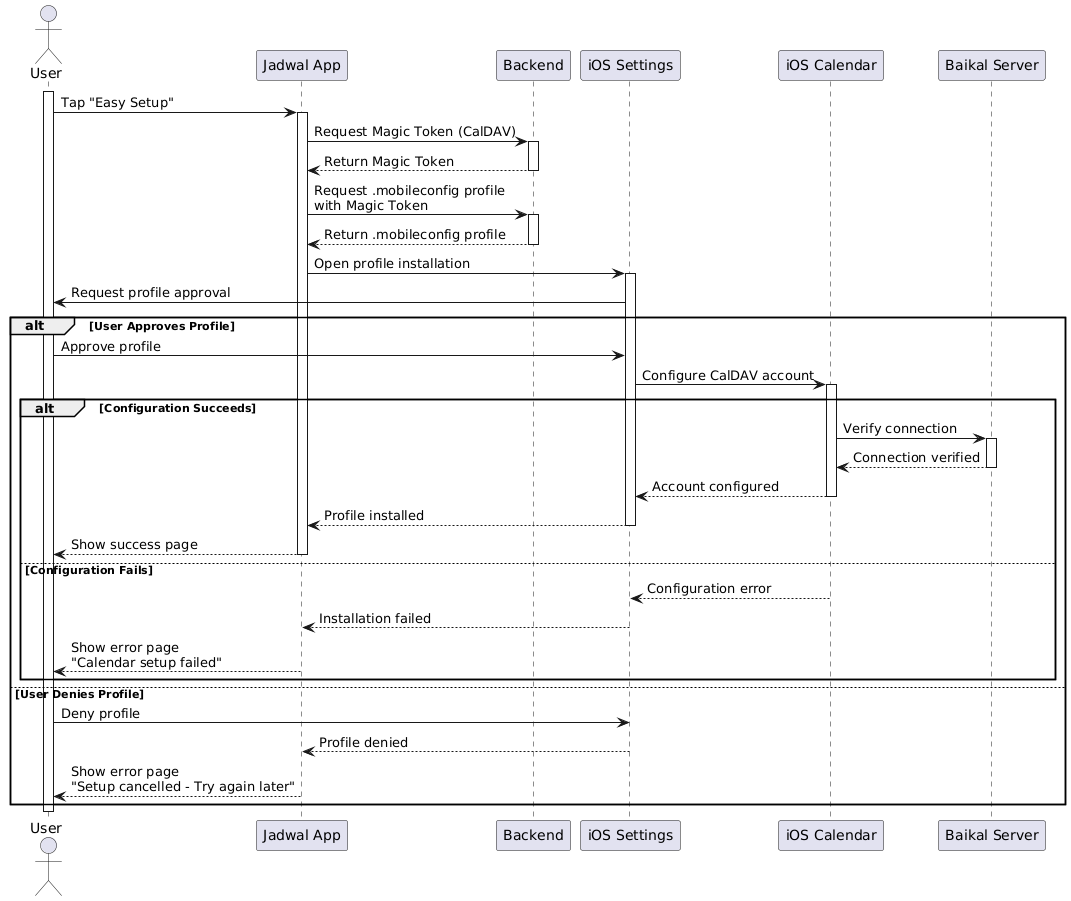
\includegraphics[width=\textwidth]{images/docs/diagrams/sequence-diagrams/all-sequence-diagrams/Connect Calendar.png}
    \caption{Connect Calendar Sequence Diagram}
    \label{fig:seq/connect-calendar}
\end{figure}

The ``Connect Calendar Sequence Diagram'', shown in \textbf{Figure~\ref{fig:seq/connect-calendar}}, illustrates the calendar integration process:

\begin{enumerate}
    \item \textbf{Local Calendar Access:} The iOS app uses EventKit framework to request and manage access to the device's calendars. This provides direct access to the user's existing calendar data.

    \item \textbf{Account Configuration:} The app retrieves encrypted CalDAV account credentials from the backend and uses iOS's native calendar system to configure the accounts. EventKit and iOS handle all direct communication with CalDAV servers, both our own and external ones.
\end{enumerate}

The Backend's role is strictly limited to securely storing and providing encrypted CalDAV account credentials. All calendar data synchronization, CalDAV communication, and event management happens through iOS's native calendar system using EventKit. This approach leverages iOS's built-in CalDAV client capabilities, ensuring reliable calendar synchronization while maintaining security of sensitive credentials.
\begin{usecase}{Create Calendar}
  \ucbasicinfo{High}{Regular}
  \ucshortdescription{This UC allows the user to create a new calendar using iOS EventKit.}
  \uctrigger{This UC is triggered when the user clicks ``Create Calendar'' in the app.}
  \ucactors{User}{EventKit}
  \ucpreconditions{
    \begin{itemize}
      \item User must be logged in
      \item Calendar access must be authorized in iOS Settings
      \item Baikal CalDAV account must be configured
    \end{itemize}
  }
  \ucrelationships{N/A}{N/A}{N/A}
  \ucinputsoutputs{
    \begin{itemize}
      \item \textbf{Calendar name} (Source: User)
      \item \textbf{Calendar account to add calendar under} (Source: User)
      \item \textbf{Calendar color} (Source: User)
    \end{itemize}
  }{
    \begin{itemize}
      \item \textbf{New calendar} (Destination: EventKit)
      \item \textbf{Creation status} (Destination: App)
    \end{itemize}
  }
  \ucmainflow{
    \begin{enumerate}
      \item The user taps the ``Calendar'' icon button in the app toolbar in the ``Calendar'' screen.
            \ucinfo{The app presents a ``Calendars'' sheet.}
      \item The user clicks the ``plus'' icon button in the toolbar of the ``Calendars'' sheet.
            \ucinfo{The app presents a form for calendar name, selector to choose account to add calendar under, and calendar color.}
      \item The user enters calendar name, selects a color, and selector to choose account to add calender under.
            \ucinfo{The app uses EventKit to create a new calendar.}
      \item EventKit creates the calendar and handles synchronization.
            \ucinfo{The calendar appears in the user's calendar list.}
    \end{enumerate}
  }
  \ucalternateflows{
    \begin{itemize}
      \item If calendar creation fails, the app shows an error and allows retry.
    \end{itemize}
  }
  \ucexceptions{
    \begin{itemize}
      \item \textbf{EventKit access denied:} The app prompts to enable calendar access in Settings.
      \item \textbf{Network issues:} EventKit handles synchronization internally.
    \end{itemize}
  }
  \ucconclusion{The UC ends when EventKit confirms the calendar creation.}
  \ucpostconditions{A new calendar is created through EventKit.}
  \ucspecialrequirements{The system must use EventKit for all calendar operations.}
\end{usecase}

\begin{figure}[!h]
  \centering
  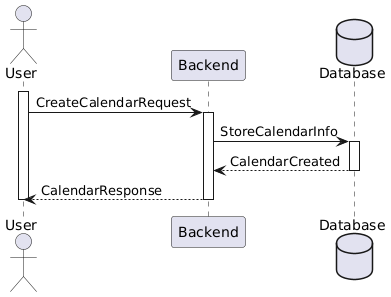
\includegraphics[width=0.5\textwidth]{images/docs/diagrams/sequence-diagrams/all-sequence-diagrams/Create Calendar.png}
  \caption{Create Calendar Sequence Diagram}
  \label{fig:seq/create-calendar}
\end{figure}

The ``Create Calendar Sequence Diagram'', shown in \textbf{Figure~\ref{fig:seq/create-calendar}}, illustrates the process of creating a new calendar in the Jadwal app. The sequence begins when the user accesses the calendar creation interface through the ``Calendars'' sheet, accessed via the calendar icon in the toolbar.

The flow involves several key steps:
\begin{enumerate}
  \item The user provides essential calendar details through a form interface:
        \begin{itemize}
          \item Calendar name
          \item Account selection (where to add the calendar)
          \item Calendar color
        \end{itemize}
  \item The app communicates with EventKit to create the new calendar
  \item EventKit handles the calendar creation and all necessary synchronization
\end{enumerate}

The process is designed to be robust and user-friendly:
\begin{itemize}
  \item If EventKit access is denied, the app guides users to enable calendar access in iOS Settings
  \item If creation fails, the app shows an error and allows retry
  \item EventKit handles all synchronization internally
\end{itemize}

This implementation leverages iOS's native EventKit framework, which manages all calendar operations and synchronization internally. This provides a reliable and native iOS experience while ensuring proper calendar management.
\begin{usecase}{View Integrated Calendar}
  \ucbasicinfo{High}{Regular}
  \ucshortdescription{Allows users to view their integrated calendar}
  \uctrigger{User selects the option to view the integrated calendar.}
  \ucactors{User}{None}
  \ucpreconditions{User must be logged into the system.}
  \ucrelationships{N/A}{N/A}{N/A}
  \ucinputsoutputs{
    \begin{itemize}
      \item \textbf{Integrated calendar} (Source: System)
    \end{itemize}
  }{
    \begin{itemize}
      \item \textbf{Integrated calendar} (Destination: App)
    \end{itemize}
  }
  \ucmainflow{
    \begin{enumerate}
      \item The user clicks on the integrated calendar.
            \ucinfo{The system displays the all integrated calendars and it's events}
    \end{enumerate}
  }
  \ucconclusion{User successfully views their integrated calendar with all the events.}
  \ucpostconditions{The integrated calendar is displayed}
  \ucspecialrequirements{N/A}
  \ucbusinessrules{
    \begin{itemize}
      \item \textbf{Events must be displayed according to user preferences .}
    \end{itemize}
  }
\end{usecase}

\begin{figure}[!h]
  \centering
  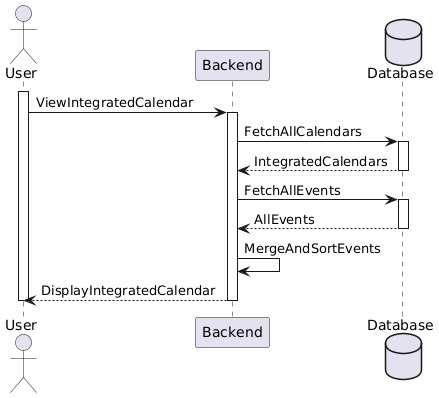
\includegraphics[width=\textwidth]{images/docs/diagrams/sequence-diagrams/all-sequence-diagrams/View Integrated Calendar.png}
  \caption{View Integrated Calendar Sequence Diagram}
  \label{fig:seq/view-integrated-calendar}
\end{figure}

The "View Integrated Calendar Sequence Diagram", shown in \textbf{Figure~\ref{fig:seq/view-integrated-calendar}}, demonstrates the process of presenting a unified view of all connected calendars to the user. The sequence begins when the user initiates a ViewIntegratedCalendar gRPC call to access their comprehensive calendar view.

The Backend executes a two-phase data retrieval process:
\begin{enumerate}
  \item First queries the Database via FetchAllCalendars to retrieve all calendar sources connected to the user's account
  \item Then executes FetchAllEvents to gather events from all calendars
\end{enumerate}

After data retrieval, the Backend performs critical processing:
\begin{itemize}
  \item Merges events from different calendar sources
  \item Sorts events chronologically
  \item Applies user preferences for event display
\end{itemize}

Finally, the Backend returns the processed calendar data through the gRPC channel as DisplayIntegratedCalendar response. This unified view ensures users can efficiently manage their schedule across all connected calendars, maintaining consistency with user preferences while providing a comprehensive overview of all commitments.

\subsection{WhatsApp Integration and Event Extraction}
One of Jadwal's key features is its ability to automatically extract events from WhatsApp conversations. These use cases explain how users connect their WhatsApp account and how the system processes messages to identify and add events to their calendar.

\begin{usecase}{Connect WhatsApp}
  \ucbasicinfo{Medium}{Regular}
  \ucshortdescription{This UC allows the user to connect their WhatsApp account to the system.}
  \uctrigger{This UC is triggered when the user clicks on ``Connect WhatsApp'' button in the app.}
  \ucactors{User}{WhatsApp}
  \ucpreconditions{User must be logged in}
  \ucrelationships{N/A}{N/A}{N/A}
  \ucinputsoutputs{
    \begin{itemize}
      \item \textbf{WhatsApp phone number} (Source: User)
      \item \textbf{WhatsApp linking code} (Source: User)
    \end{itemize}
  }{
    \begin{itemize}
      \item \textbf{WhatsApp auth credentials} (Destination: System)
    \end{itemize}
  }
  \ucmainflow{
    \begin{enumerate}
      \item The user clicks ``Connect WhatsApp'' button.
            \ucinfo{The system asks for the user's WhatsApp phone number.}
      \item The user enters their WhatsApp phone number.
            \ucinfo{WhatsApp shows the linking code in their app.}
      \item The user enters the linking code in our app.
            \ucinfo{The app shows a success screen if connection was sucessful.}
    \end{enumerate}
  }
  \ucalternateflows{
    \begin{itemize}
      \item If the WhatsApp connection fails, the user must redo the steps and try again.
      \item If the user enters a wrong linking code, the connection of the WhatsApp account will fail unless they enter the correct code.
    \end{itemize}
  }
  \ucexceptions{
    \begin{itemize}
      \item \textbf{Wrong linking code:} If the user enters a wrong linking code too many times, the connection of the WhatsApp account will fail.
      \item \textbf{Network issue:} A network issue interrupting the communication between the app, the server, and WhatsApp.
    \end{itemize}
  }
  \ucconclusion{The UC ends when the user has a connected WhatsApp account in the system.}
  \ucpostconditions{The system has access to the user's WhatsApp account.}
\end{usecase}

\begin{figure}[!h]
  \centering
  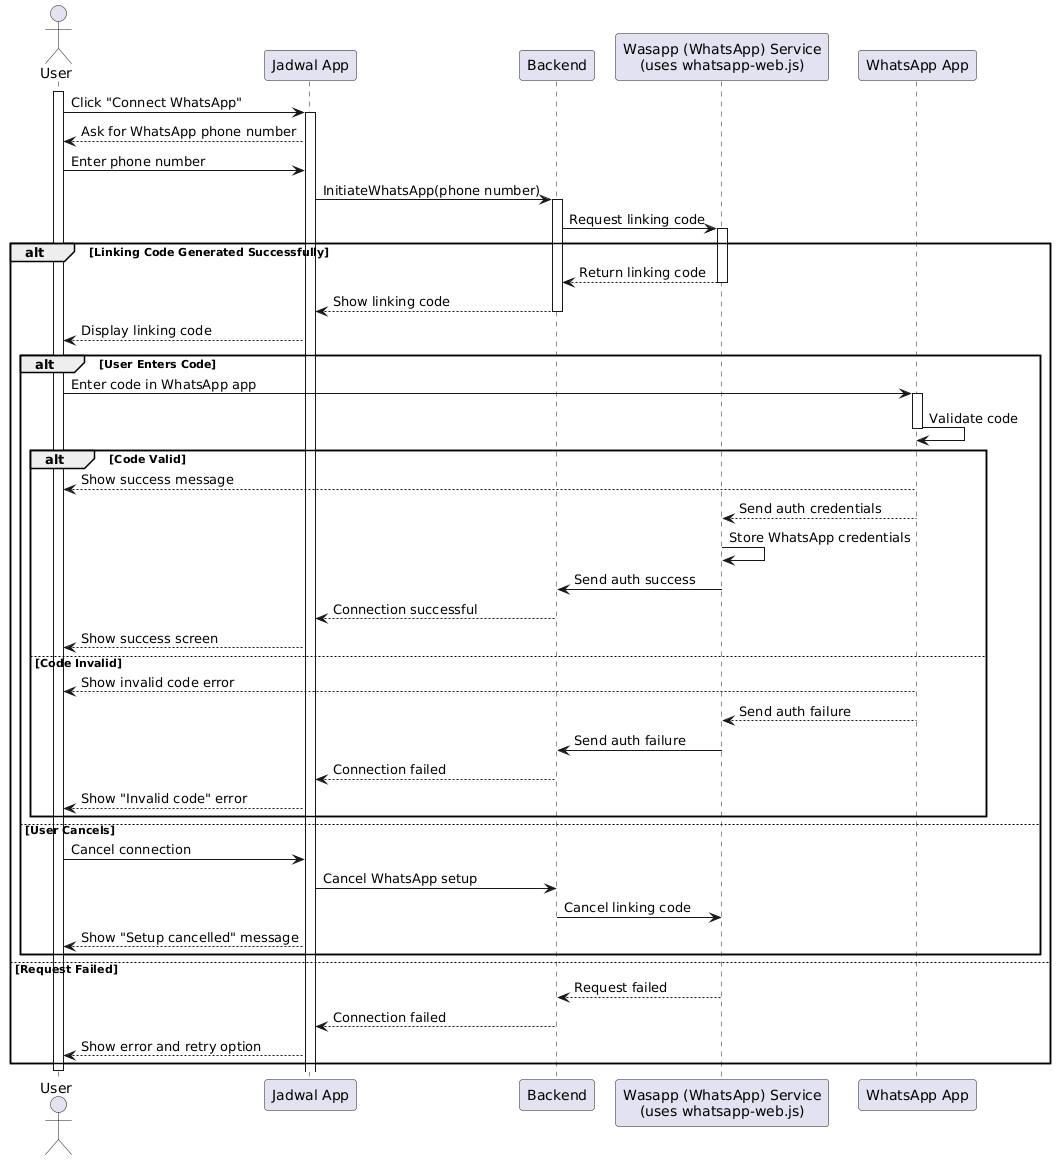
\includegraphics[width=\textwidth]{images/docs/diagrams/sequence-diagrams/all-sequence-diagrams/Connect WhatsApp.png}
  \caption{Connect WhatsApp Sequence Diagram}
  \label{fig:seq/connect-whatsapp}
\end{figure}

The "Connect WhatsApp Sequence Diagram", shown in \textbf{Figure~\ref{fig:seq/connect-whatsapp}}, illustrates the two-phase authentication process for connecting a user's WhatsApp account to Jadwal. The sequence begins with the InitiateWhatsApp gRPC call, where the user provides their phone number to the Backend.

The Backend then communicates with the WhatsApp service to request a linking code. This interaction follows two possible paths:

\begin{itemize}
  \item If the linking code request succeeds:
        \begin{enumerate}
          \item The user receives the linking code in their WhatsApp application
          \item The user initiates the CompleteWhatsApp gRPC call with the linking code
          \item The Backend validates the code with WhatsApp
          \item Upon successful validation, the WhatsApp authentication credentials are securely stored in the Database for future use
        \end{enumerate}
  \item If the linking code request fails:
        \begin{itemize}
          \item The Backend immediately returns an InitiateWhatsApp failure response to the user
        \end{itemize}
\end{itemize}

During the completion phase, if the linking code validation fails, the Backend returns a CompleteWhatsApp failure response, requiring the user to restart the process. This secure two-phase authentication ensures that only legitimate WhatsApp account owners can connect their accounts to Jadwal while maintaining the integrity of the WhatsApp integration.
\clearpage
\begin{usecase}{Extract Events from WhatsApp}
  \ucbasicinfo{High}{Regular}
  \ucshortdescription{Allows users to extract event details shared in WhatsApp messages and save them to their calendar.}
  \uctrigger{User selects a message containing event details in WhatsApp.}
  \ucactors{User}{WhatsApp}
  \ucpreconditions{User must have WhatsApp installed and linked to the system.}
  \ucrelationships{N/A}{Event Management}{N/A}
  \ucinputsoutputs{
    \begin{itemize}
      \item \textbf{User-selected WhatsApp message containing event details.} (Source: User)
    \end{itemize}
  }{
    \begin{itemize}
      \item \textbf{Extracted event details saved to the calendar.} (Destination: User)
    \end{itemize}
  }
  \ucmainflow{
    \begin{enumerate}
      \item User opens WhatsApp and selects a message with event details. 
        \ucinfo{Display of the selected message.}
      \item User taps on the ``Extract Event'' option.
        \ucinfo{System processes the message to identify event details.}
      \item System extracts event details from the message.
        \ucinfo{Date, time, and location are parsed from the text. }
    \end{enumerate}
  }
  \ucalternateflows{
    \begin{itemize}
      \item If the message does not contain valid event details, display an error message.
      \item Notify the user about invalid format. 
    \end{itemize}
  }
  \ucexceptions{
    \begin{itemize}
      \item If there is a system error during extraction, display a relevant error message. 
      \item Log error for troubleshooting.
    \end{itemize}
  }
  \ucconclusion{User successfully extracts event details from WhatsApp and saves them to the calendar.}
  \ucpostconditions{The event is added to the user's calendar, and the user can view it in their schedule.}
  \ucbusinessrules{
    \begin{itemize}
      \item Only messages with recognized event formats can be extracted.
    \end{itemize}
  }
  \ucspecialrequirements{The system must have permissions to access WhatsApp messages and extract relevant information.}
\end{usecase}

\subsection{Event Management and Conflict Resolution}
Managing events and resolving scheduling conflicts are daily challenges for users. These use cases demonstrate how Jadwal handles event creation, conflict detection, and provides smart resolution options.

\begin{usecase}{Suggest Conflict Resolutions}
  \ucbasicinfo{HIGH}{Regular}
  \ucshortdescription{This UC gives the user all the conflicts and possible ways to resolve it.}
  \uctrigger{The UC is triggered when a conflict is detected between any overlapping event}
  \ucactors{User}{Calendar System, WhatsApp}
  \ucpreconditions{The calendar must have events}
  \ucrelationships{None}{Manage Scheduling Conflicts}{None}
  \ucinputsoutputs{
    \begin{itemize}
      \item Overlapping events (Source: User or WhatsApp extraction)
      \item User suggested resolution (Source: User)
    \end{itemize}
  }{
    \begin{itemize}
      \item {Resolution options} (Destination: User Interface)
      \item {Updated calendar schedule} (Destination: Calendar)
    \end{itemize}
  }
  \ucmainflow{
    \begin{enumerate}
      \item Conflict Detection  
        \ucinfo{The system detects overlapping of events either added manually or extracted from WhatsApp.}
      \item Offer Resolutions
        \ucinfo{The system provides the user with the list of resolution options.
        \begin{itemize}
          \item By moving the overlapping event to another time slot.   
          \item Keep both events with a conflict warning. 
        \end{itemize}}
      \item User Selection  
        \ucinfo{The user moves the overlapping event to another time slot by the list provided by the system}
      \item Implement Resolution
        \ucinfo{The system makes the changes in the calendar respectively}
    \end{enumerate}
  }
  \ucalternateflows{
    \begin{enumerate}
      \item {N/A}
    \end{enumerate}
  }
  \ucexceptions{
    \begin{itemize}
      \item If the system doesn't get any possible way to resolve the conflict then the system would mark both the event as conflicting or displays to delete one of the event.
      \item If the user doesn't choose any option to resolve the conflict then both the events are makrd as conflicting.
    \end{itemize}
  }
  \ucconclusion{The UC ends when the user gives it's input for resolution weather if it's to reschedule the event, delete it or leave it without resolving and it is reflected in on the calendar.}
  \ucpostconditions{The conflicting events in the calendar are either resolved or marked as conflicting}
  \ucspecialrequirements{The system give feasible conflict resolution options}
\end{usecase}

\begin{usecase}{Manage Scheduling Conflicts}
  \ucbasicinfo{Medium}{Regular}
  \ucshortdescription{This UC allows the user to manage scheduling conflicts by suggesting resolutions when overlapping events are detected.}
  \uctrigger{This UC is triggered when an automatically added event overlaps with an existing event.}
  \ucactors{User}{None}
  \ucpreconditions{
    \begin{itemize}
      \item User is logged in.
      \item Conflicting events list is not empty.
    \end{itemize}
  }
  \ucrelationships{N/A}{N/A}{N/A}
  \ucinputsoutputs{
    \begin{itemize}
      \item \textbf{Conflicting events} (Source: System)
      \item \textbf{Event to override} (Source: User)
    \end{itemize}
  }{
    \begin{itemize}
      \item \textbf{Conflict resolution suggestion} (Destination: User Interface)
      \item \textbf{Updated event schedules} (Destination: Calendar)
    \end{itemize}
  }
  \ucmainflow{
    \begin{enumerate}
      \item The user opens the application and clicks on the view conflicts icon
        \ucinfo{The application shows all the conflics with their resolution options}
      \item The user chooses the best fit option to manage each conflict 
        \ucinfo{The conflict is resolved and is removed from the conflict list }

    \end{enumerate}
  }
  \ucalternateflows{
    \begin{enumerate}
      \item If the user doesn't choose any option, it shows conflicting status until the user chooses any option or the event expires. 
      \item If the user clicks on reject the event is left overlapping.
    \end{enumerate}
  }
  \ucexceptions{
    \begin{itemize}
      \item Netwok failure 
    \end{itemize}
  }
  \ucconclusion{The UC ends when the conflicting events are either resolved or marked as conflicting, based on the user's choice.}
  \ucpostconditions{The calendar reflects the user's decision regarding event conflicts.}
  \ucspecialrequirements{The system should provide best suggestions for resolving conflicts.}
\end{usecase}

\begin{figure}[!h]
  \centering
  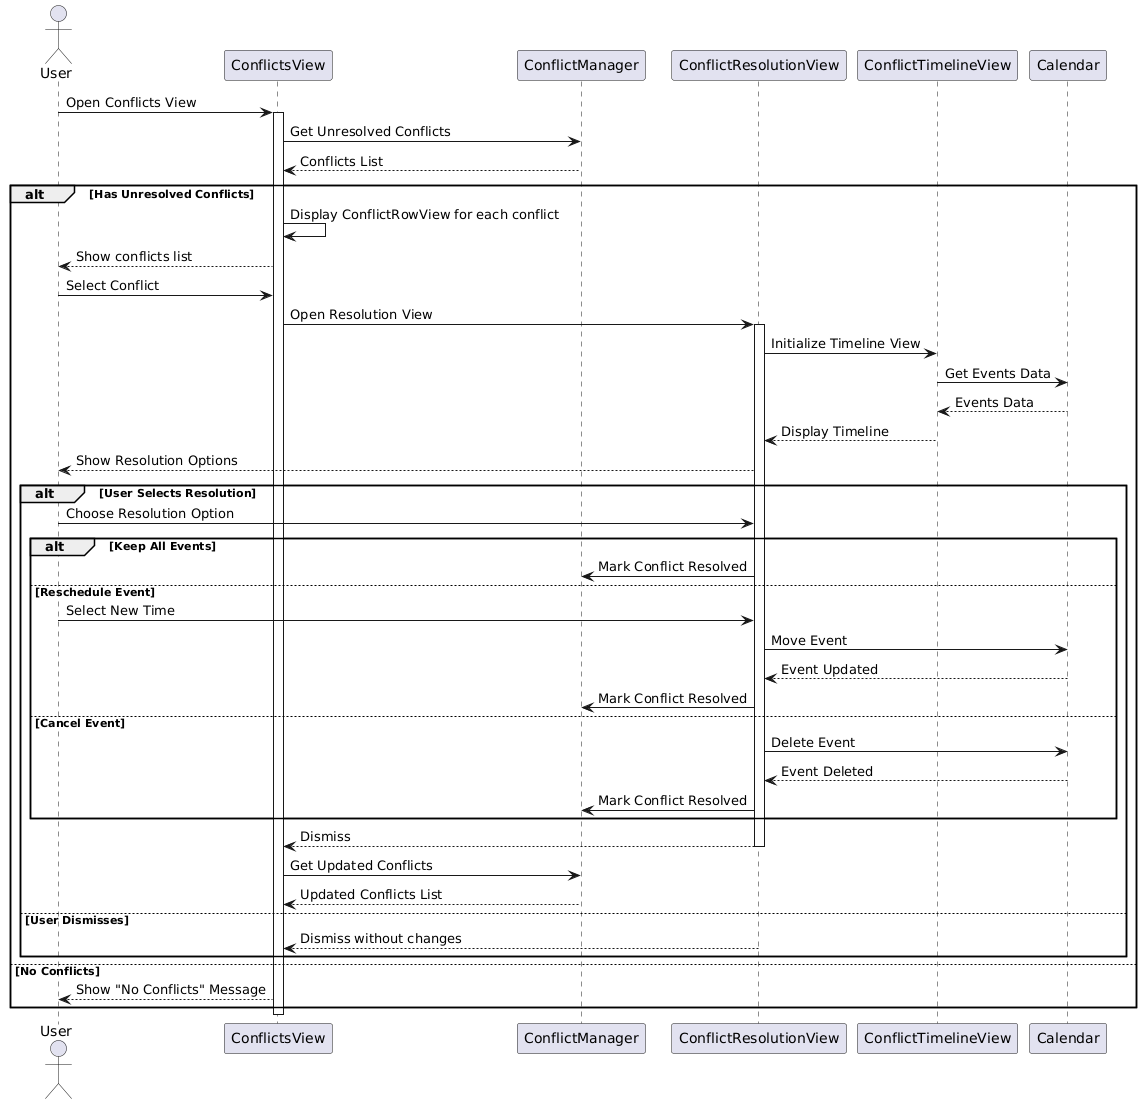
\includegraphics[width=\textwidth]{images/docs/diagrams/sequence-diagrams/all-sequence-diagrams/Manage Scheduling Conflicts.png}
  \caption{Manage Scheduling Conflicts Sequence Diagram}
  \label{fig:seq/manage-scheduling-conflicts}
\end{figure}
\begin{usecase}{Add Event Manually}
    \ucbasicinfo{High}{Regular}
    \ucshortdescription{This UC allows users to add events manually }
    \uctrigger{The user clicks and adds the events.}
    \ucactors{User}{None}
    \ucpreconditions{The user is logged into the application }
    \ucrelationships{N/Al}{N/A}{N/A}
    \ucinputsoutputs{
      \begin{itemize}
        \item \textbf{Event Name} (Source: User)
        \item \textbf{Event Location} (Source: User)
        \item \textbf{Event Date (Start and End)} (Source: User)
        \item \textbf{Event Time (Start and End)} (Source: User)
        \item \textbf{Event Description} (Source: User)
        \item \textbf{Notifications/Reminders} (Source: User)
      \end{itemize}
    }{
      \begin{itemize}
        \item \textbf{The event is displayed on the calendar with its details and duration
        } (Destination: Calendar)
      \end{itemize}
    }
    \ucmainflow{
      \begin{enumerate}
        \item The name of the event (e.g., ``Meeting with Client'')
          \ucinfo{Event is saved and displayed on the user’s calendar}
        \item The start and end time of the event.
          \ucinfo{The system displays the event in the correct time slot with its duration, while checking for conflicts and scheduling notifications}
        \item The User optionally adds a description
          \ucinfo{The system stores and displays description of the event.}
        \item Set reminders for the event.
          \ucinfo{Notification or reminder set for the event}
      \end{enumerate}
    }
    \ucalternateflows{
      \begin{enumerate}
        \item User clicks on a date on the calendar to bring up a popup with event fields and the date is pre-filled. 
        \item	The user can add a different color for the events.
      \end{enumerate}
    }
    \ucexceptions{
      \begin{itemize}
        \item Invalid date and time format\
        \item The event's start and end times conflict with an existing event
        \item The user attempts to save the event without filling in mandatory fields
      \end{itemize}
    }
    \ucconclusion{The UC ends when the event has been successfully added to the calendar, and the user sees it displayed.}
    \ucpostconditions{The event is successfully added to the calendar, visible in the correct time slot, and notifications are set as per user preferences}
    \ucspecialrequirements{The interface must be simple and allowing users to input events with less efforts.}
\end{usecase}

\subsection{Prayer Time and Notification Management}
Prayer time scheduling is a unique feature of Jadwal, and timely notifications ensure users never miss important events. These use cases detail how prayer times are scheduled and how the notification system keeps users informed.

\begin{usecase}{Schedule Prayer Times}
    \ucbasicinfo{High}{Regular}
    \ucshortdescription{Allows users to create, edit, and manage their prayer time schedules.}
    \uctrigger{User selects the option to schedule prayer times.}
    \ucactors{User}{None}
    \ucpreconditions{User must be logged into the system.}
    \ucrelationships{N/A}{N/A}{N/A}
    \ucinputsoutputs{
      \begin{itemize}
        \item \textbf{User's prayer time details} (Source: user)
        \item \textbf{(date, time)}
      \end{itemize}
    }{
      \begin{itemize}
        \item \textbf{Confirmation of scheduled prayer times, calendar entries.}
      \end{itemize}
    }
    \ucmainflow{
      \begin{enumerate}
        \item User navigates to the prayer scheduling page.
          \ucinfo{User is presented with a form to enter prayer times. Display of the scheduling interface.}
        \item User inputs prayer time details.
          \ucinfo{Input fields for time, date, and prayer type. User's input is captured for validation.}
        \item User saves the schedule.
          \ucinfo{System checks for valid input. Confirmation message displayed.}
        \item System confirms schedule creation.
          \ucinfo{User receives a notification. Scheduled prayer times are saved in the system.}
      \end{enumerate}
    }
    \ucalternateflows{
      \begin{itemize}
        \item If input is invalid, display error messages.
      \end{itemize}
    }
    \ucexceptions{
      \begin{itemize}
        \item If there's a system error, display a relevant error message.
      \end{itemize}
    }
    \ucpostconditions{The system generates calendar entries for the scheduled prayer times.}
    \ucspecialrequirements{The system must support notifications for prayer times.}
    \ucconclusion{User's prayer times are successfully scheduled.}
    \ucbusinessrules{
      \begin{itemize}
        \item Prayer times must be within valid time ranges.
      \end{itemize}
    }
\end{usecase}
\begin{usecase}{Receive Event Notifications}
  \ucbasicinfo{High}{Regular}
  \ucshortdescription{Users receive notifications about upcoming events.}
  \uctrigger{The UC is triggered when the choosen time of an event's reminder has arrived}
  \ucactors{User}{None}
  \ucpreconditions{User must be logged into the system and set a reminder of the specific event.}
  \ucrelationships{N/A}{N/A}{N/A}
  \ucinputsoutputs{
    \begin{itemize}
      \item \textbf{Time of the event reminder} (Source: User)
    \end{itemize}
  }{
    \begin{itemize}

      \item \textbf{Notifications sent to users.} (Destination: System)
    \end{itemize}
  }
  \ucmainflow{
    \begin{enumerate}
      \item The system checks the alarms set for every event.
            \ucinfo{The system checks every 1 minute for set alarms for every event.}
      \item Notifications sent to users.
            \ucinfo{The user is reminded about the event by sending the notification}
    \end{enumerate}
  }
  \ucalternateflows{
    \begin{itemize}
      \item \textbf{If user denys the access to the notification the notifications are not sent.}
    \end{itemize}
  }
  \ucexceptions{
    \begin{itemize}
      \item \textbf{Netwok issue}
    \end{itemize}
  }
  \ucconclusion{The system checks for set alarm every 1 minute and if the event is detected the system sends the notification.}
  \ucpostconditions{Notifications are sent.}
  \ucspecialrequirements{Notification permission.}
  \ucbusinessrules{The system has to check every minute for the set alarm.
  }
\end{usecase}

\begin{figure}[!h]
  \centering
  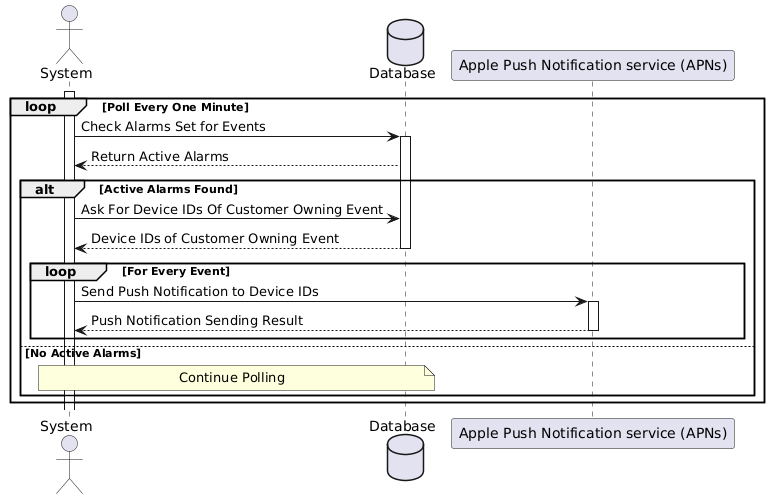
\includegraphics[width=\textwidth]{images/docs/diagrams/sequence-diagrams/all-sequence-diagrams/Receive Event Notifications.png}
  \caption{Receive Event Notifications Sequence Diagram}
  \label{fig:seq/receive-event-notifications}
\end{figure}

The ``Receive Event Notifications Sequence Diagram'', shown in \textbf{Figure~\ref{fig:seq/receive-event-notifications}}, illustrates Jadwal's continuous event notification monitoring and delivery system. The sequence operates in a continuous polling loop that executes every minute, ensuring timely notification delivery for all scheduled events.

The polling process consists of several key steps:
\begin{enumerate}
  \item The System queries the Database for active alarms through regular checks
  \item For each batch of active alarms found:
        \begin{itemize}
          \item Retrieves associated device IDs for notification targets
          \item Iterates through each event requiring notification
          \item Dispatches push notifications via Apple Push Notification service (APNs)
        \end{itemize}
  \item If no active alarms are found, the system continues its polling cycle
\end{enumerate}

This robust notification system ensures reliable delivery of event reminders while efficiently managing system resources. The one-minute polling interval provides a balance between timely notifications and system performance, while the batch processing of notifications optimizes the interaction with APNs. The system's ability to handle multiple device IDs per user ensures notifications reach users across all their registered devices.

% ==========

\section{Activity Diagram}

\begin{figure}[!h]
    \centering
    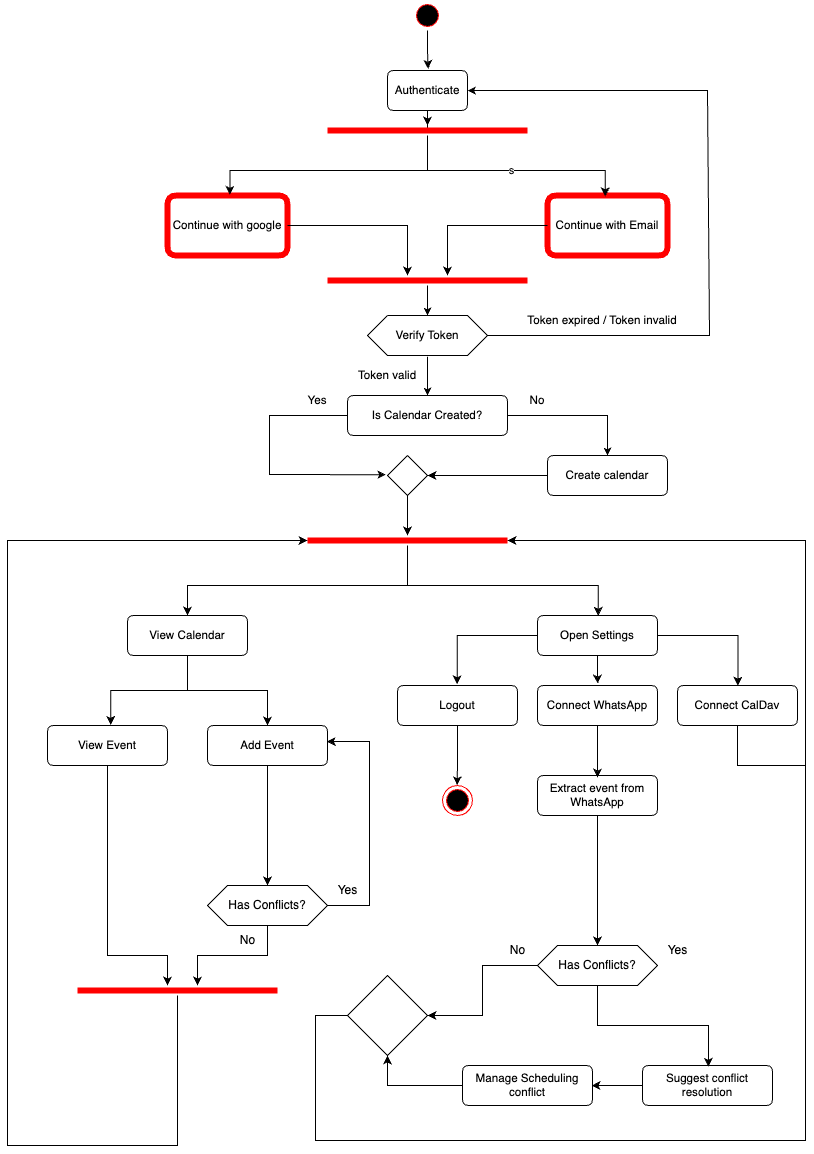
\includegraphics[width=0.9\textwidth]{images/activity-diagram.png}
    \caption{Activity Diagram of Jadwal}
    \label{fig:activity-diagram}
\end{figure}

\newpage

An activity diagram is shown in Figure~\ref{fig:activity-diagram} above, and it illustartes the flows the user of the app can take. It starts with the authentication whcih supports both Google and Email. Then afater the token is verified, a check is done to see if the user has a calendar or not. If the user has a calendar, we just move on, but if they don't have one, we create one and then move on. Here the user is inside the app and has two options, he can either view the calendar or open the settings page. When he views the calendar, he can view an event, or add one. Adding event might result in a conflict, so if one arises, they can try editing it and adding it again til no conflicts arise. After any of those two steps, the user can go back to view calendar or open settings page. If the choose to open settings page, they have three actions available. They can connect a CalDAV account, connect WhatsApp, or logout. Starting with the connecting a WhatsApp account, the system will extract events from the user's WhatsApp account automatically. If any conflicts arise, the system suggests a conflict resolution, and the user can take action by managing the scheduling conflict. But if no conflicts arise, the system just continues normally. Another option for the user is connecting a CalDAV account, and once that happens, the user can go back to having the option of going to calendar view or open settings page. Finally, the logout action and that terminates the session and the user is logged out of the app.



\section{Class Diagram}

The figures below show the main classes Jadwal's system includes. The figures give an overview of interfaces in the system to help in understanding the different parts of the system. Since Golang will be used for the backend mainly, the diagrams below are more suited for it.

Of course that doesn't mean they can't be used for implementing in other languages, but the way it was written took into consideration the language features. Golang is neither fully object oriented neither fully functional. It has \texttt{interface} and \texttt{struct}, and has implicit implementation. Implicit implementation means as long as a struct has the methods that an interface expects, that struct implemented the interface. Below is a key for the class diagrams coming below:
\begin{itemize}
    \item S - \texttt{struct} (Go struct type)
    \item T - \texttt{type} (Go type definition)
    \item C - \texttt{class} (Go interface implementations)
    \item I - \texttt{interface} (Go interface definition)
\end{itemize}

\newpage

\begin{figure}[!h]
    \centering
    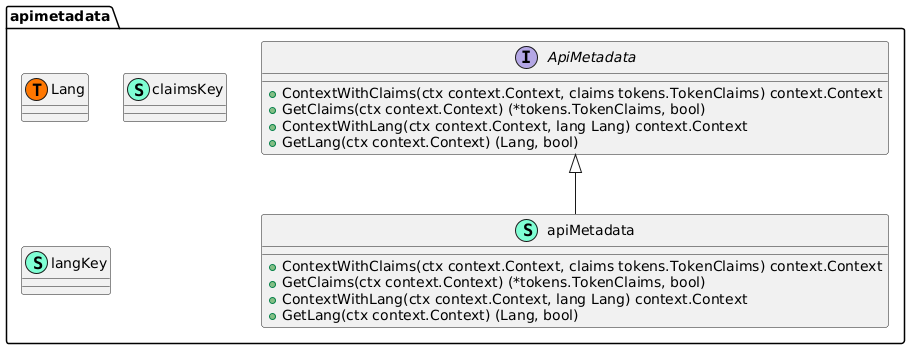
\includegraphics[width=0.9\textwidth]{images/docs/diagrams/class/class-diagram/apimetadata.png}
    \caption{Api Metadata Class Diagram}
    \label{fig:api-metadata-class-diagram}
\end{figure}

In Figure~\ref{fig:api-metadata-class-diagram}, the diagram shows the Api Metadata interface and its implementation along with important fields. It basically extracts data from the headers and includes it in the context of the requests. It helps you put stuff into the context and extract it from them. Context in Golang allows you to attach stuff to it, but it is not type safe, so we are making a wrapper to make it safe. Below we are adding wrappers for \texttt{Claims} and \texttt{Lang}. \texttt{Claims} are extracted from the JWT (JSON Web Token). \texttt{Lang} is self-explanatory.

\newpage

\begin{figure}[!h]
    \centering
    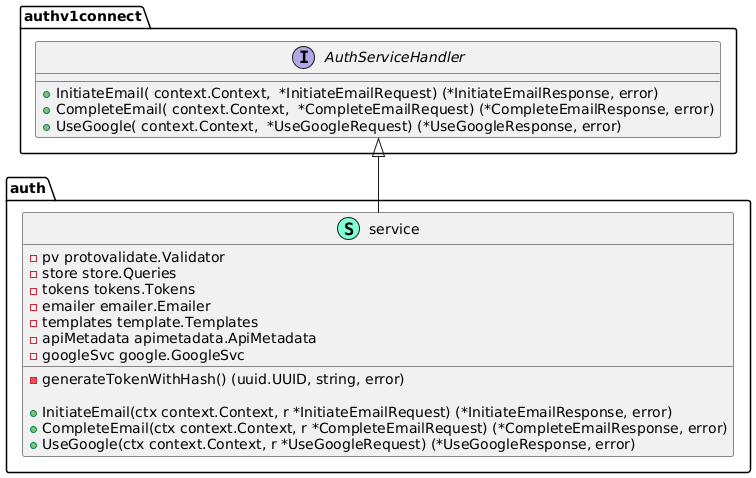
\includegraphics[width=0.9\textwidth]{images/docs/diagrams/class/class-diagram/auth.png}
    \caption{Auth Class Diagram}
    \label{fig:auth-class-diagram}
\end{figure}

In Figure~\ref{fig:auth-class-diagram}, the diagram shows the Auth API interface with its dependencies.
It also shows the \texttt{authv1connect} which is the generated code for the API\@.
This includes the flow for using email to authenticate and using Google.

\newpage

\begin{figure}[!h]
    \centering
    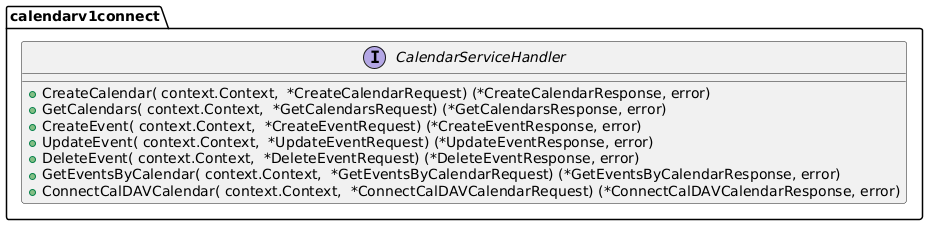
\includegraphics[width=0.9\textwidth]{images/docs/diagrams/class/class-diagram/calendarv1.png}
    \caption{Calendar V1 Class Diagram}
    \label{fig:calendar-v1-class-diagram}
\end{figure}

In Figure~\ref{fig:calendar-v1-class-diagram}, the diagram shows the api layer service calendar.
It allows Jadwal's clients to manage their calendar data easily.
It shows the interfaces and the implementation structs with their fields and methods.

\newpage

\begin{figure}[!h]
    \centering
    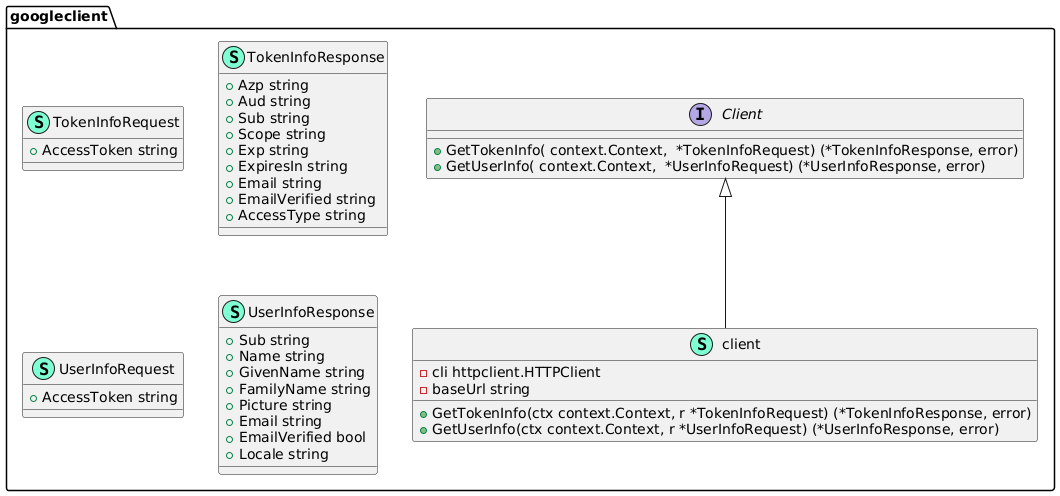
\includegraphics[width=0.9\textwidth]{images/docs/diagrams/class/class-diagram/googleclient.png}
    \caption{Google Client Class Diagram}
    \label{fig:googleclient-class-diagram}
\end{figure}

In Figure~\ref{fig:googleclient-class-diagram}, the Google client, and its methods.
It allows Jadawl to verify with Google that tokens its gets are good, and it also allows Jadwal system to get the user info the system was granted access for.

\newpage

\begin{figure}[!h]
    \centering
    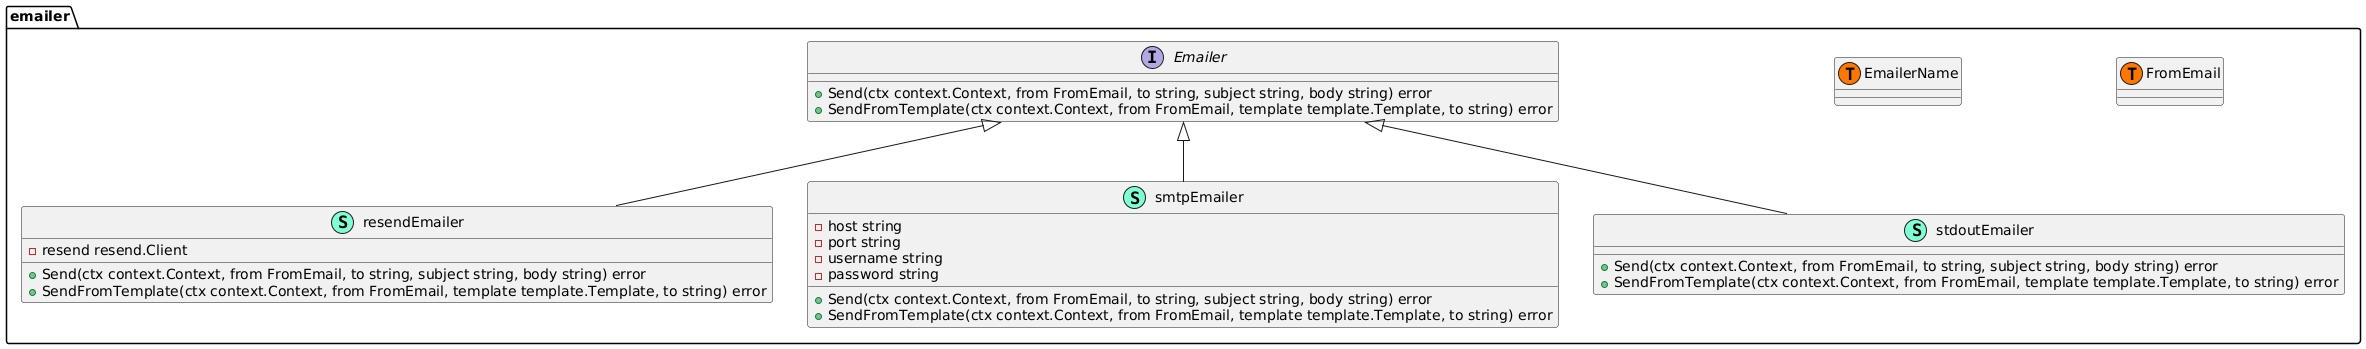
\includegraphics[width=0.9\textwidth]{images/docs/diagrams/class/class-diagram/emailer.png}
    \caption{Emailer Class Diagram}
    \label{fig:emailer-class-diagram}
\end{figure}

In Figure~\ref{fig:emailer-class-diagram}, the diagram shows the \texttt{emailer} interface with its three implementations. This allows for using the texttt{stdoutEmailer} when testing locally, and using either of the \texttt{resendEmailer} or \texttt{smtpEmailer} in production to send real emails.

\newpage

\begin{figure}[!h]
    \centering
    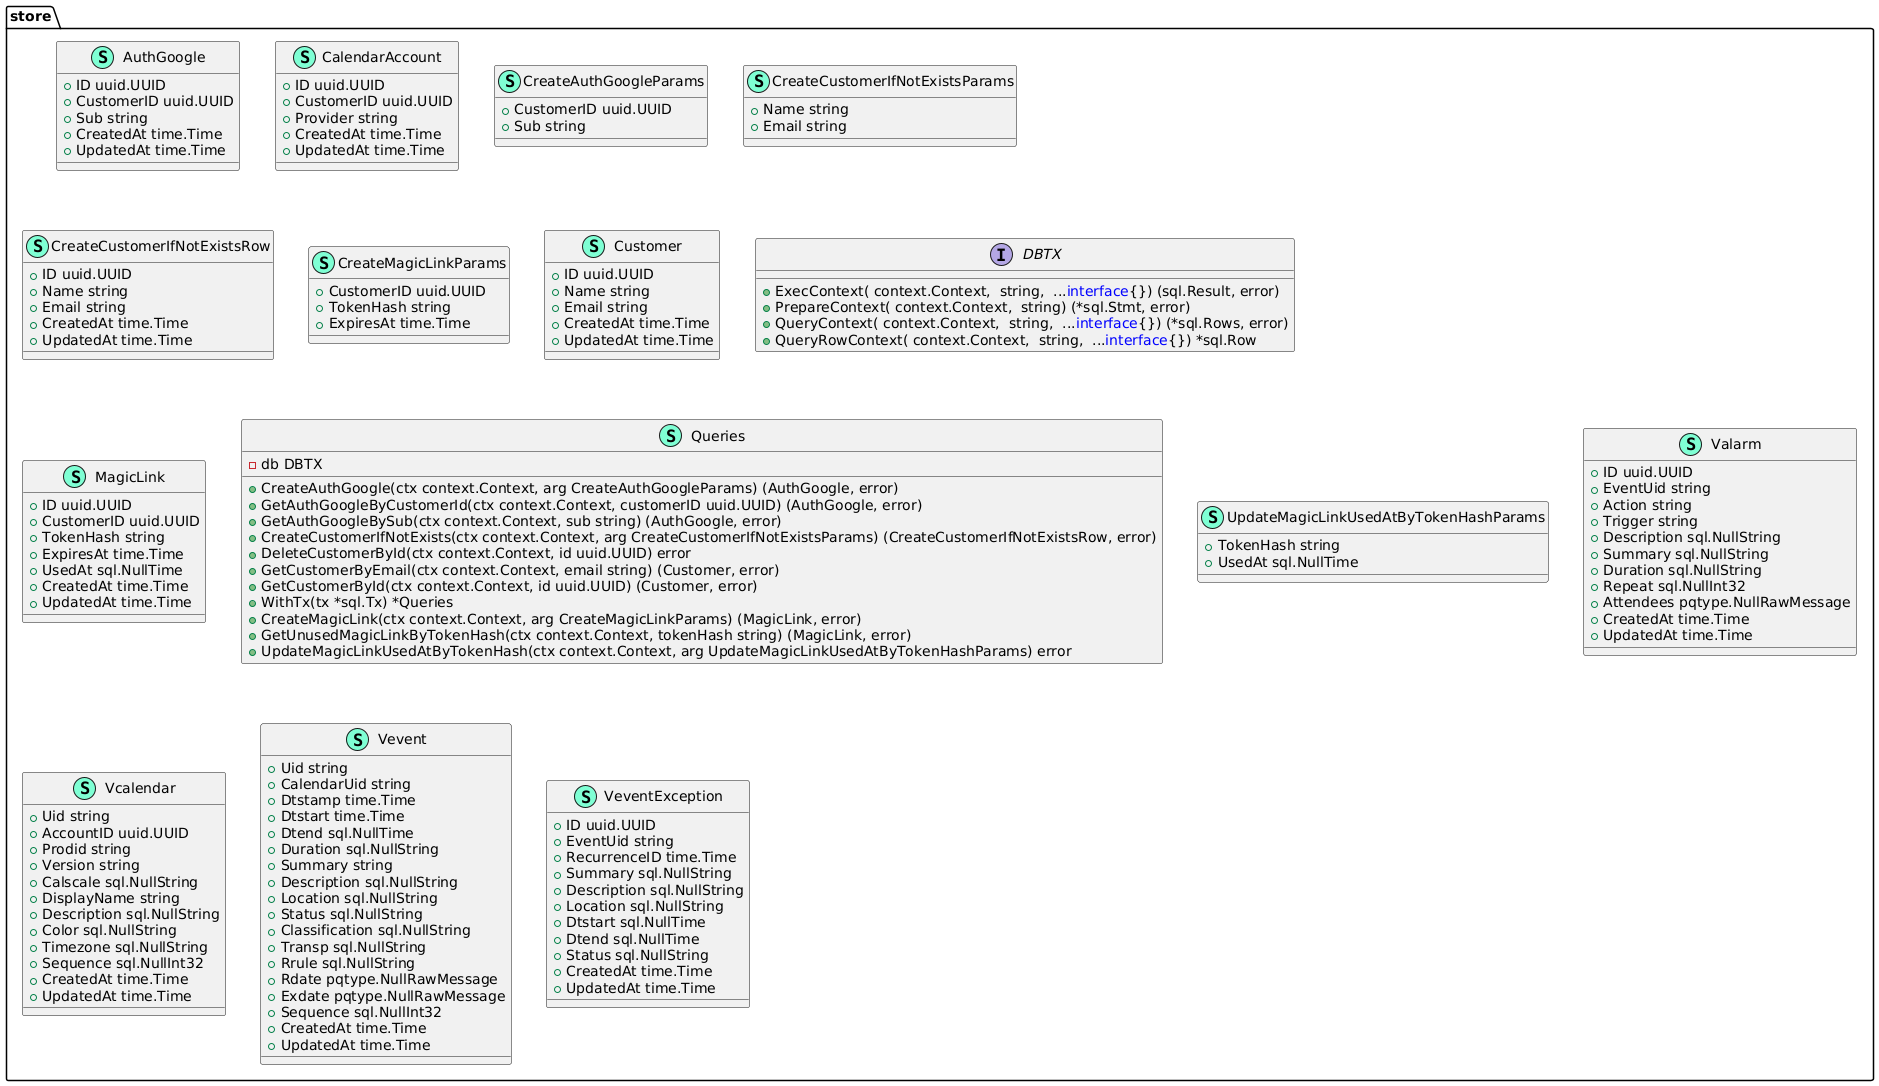
\includegraphics[width=0.9\textwidth]{images/docs/diagrams/class/class-diagram/store.png}
    \caption{Store Class Diagram}
    \label{fig:store-class-diagram}
\end{figure}

In Figure~\ref{fig:store-class-diagram}, the diagram shows the store, or in other words the database. The store holds all the methods needed to query the database for information it holds. More methods can be added as needed, but those are the core methods.

\newpage

\begin{figure}[!h]
    \centering
    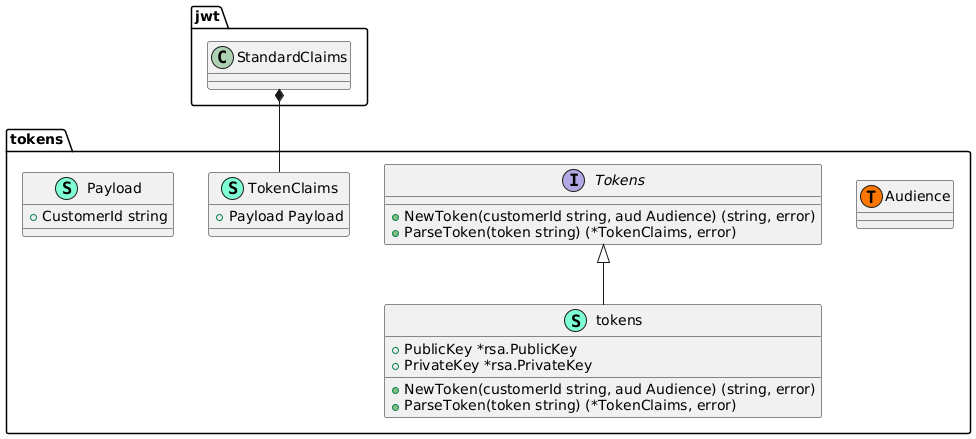
\includegraphics[width=0.9\textwidth]{images/docs/diagrams/class/class-diagram/tokens.png}
    \caption{Tokens Class Diagram}
    \label{fig:tokens-class-diagram}
\end{figure}

In Figure~\ref{fig:tokens-class-diagram}, the diagram shows the tokens service implementation along with its interface. The diagram also illustartes the needed \texttt{struct} representation for any data passed to and from the service.

\newpage

\begin{figure}[!h]
    \centering
    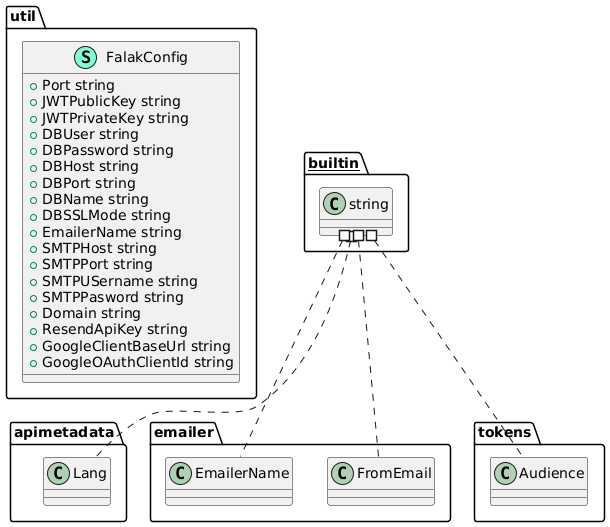
\includegraphics[width=0.5\textwidth]{images/docs/diagrams/class/class-diagram/util.png}
    \caption{Util Class Diagram}
    \label{fig:util-class-diagram}
\end{figure}

In Figure~\ref{fig:util-class-diagram}, the diagram shows config needed to support both production and development without committing secrets to the codebase. Falak in this context is the codename for the backend. The config here is represented as a \texttt{struct} since it is hold data and doesn't need implementations.

\section{Database Design}

The foundation of Jadwal's robust functionality lies in its carefully structured relational database architecture. This section presents both the Entity-Relationship model and Relational Schema that support the application's core features, from user authentication to calendar integration and event management. The database design ensures efficient data organization while maintaining the flexibility needed for future scalability.

\subsection{Entity-Relationship Model}

The Entity-Relationship model, illustrated in \textbf{Figure~\ref{fig:er-diagram}}, depicts the conceptual structure of Jadwal's database system. This model follows standard ER notation and demonstrates the relationships between the system's primary entities.

\subsubsection{Core Entities and Relationships}

\begin{enumerate}
    \item \textbf{User Management}
          \begin{itemize}
              \item \texttt{customer}: Central entity with attributes \texttt{id} (UUID), \texttt{name}, and \texttt{email}
              \item \texttt{auth\_google}: Represents Google OAuth authentication
              \item \texttt{magic\_link}: Manages email-based authentication tokens
          \end{itemize}

    \item \textbf{Calendar Organization}
          \begin{itemize}
              \item \texttt{calendar\_accounts}: Links customers to calendar providers
              \item \texttt{vcalendar}: Represents individual calendars with metadata
              \item One-to-many relationship from accounts to calendars
          \end{itemize}

    \item \textbf{Event Management}
          \begin{itemize}
              \item \texttt{vevent}: Core event entity with timing and details
              \item \texttt{vevent\_exception}: Handles recurring event modifications
              \item \texttt{valarm}: Manages event notifications
          \end{itemize}
\end{enumerate}

\subsubsection{Key Relationships}

\begin{itemize}
    \item Customer "has" authentication methods (one-to-many)
    \item Customer "owns" calendar accounts (one-to-many)
    \item Calendar accounts "contain" calendars (one-to-many)
    \item Calendars "schedule" events (one-to-many)
    \item Events "have" exceptions and alarms (one-to-many)
\end{itemize}

\subsection{Relational Database Schema}

The relational database schema, shown in \textbf{Figure~\ref{fig:relational-schema}}, provides the detailed logical structure of the database implementation. This representation demonstrates the actual table structures, attributes, and relationships as implemented in the database system.

\subsubsection{Table Structures}

\begin{enumerate}
    \item \textbf{Authentication Tables}
          \begin{itemize}
              \item \texttt{customer} (\underline{id}, name, email, created\_at, updated\_at)
              \item \texttt{auth\_google} (\underline{id}, customer\_id, sub, created\_at, updated\_at)
              \item \texttt{magic\_link} (\underline{id}, customer\_id, token\_hash, expires\_at, used\_at, created\_at, updated\_at)
          \end{itemize}

    \item \textbf{Calendar Tables}
          \begin{itemize}
              \item \texttt{calendar\_accounts} (\underline{id}, customer\_id, provider, created\_at, updated\_at)
              \item \texttt{vcalendar} (\underline{uid}, account\_id, prodid, version, display\_name, description, color, timezone, created\_at, updated\_at)
          \end{itemize}

    \item \textbf{Event Tables}
          \begin{itemize}
              \item \texttt{vevent} (\underline{uid}, calendar\_uid, dtstamp, dtstart, dtend, duration, summary, location, status, classification, transp, rrule, rdate, exdate, sequence, created\_at, updated\_at)
              \item \texttt{vevent\_exception} (\underline{id}, event\_uid, recurrence\_id, summary, description, location, dtstart, dtend, status, created\_at, updated\_at)
              \item \texttt{valarm} (\underline{id}, event\_uid, action, trigger, description, summary, duration, repeat, attendees, created\_at, updated\_at)
          \end{itemize}
\end{enumerate}

\subsubsection{Implementation Details}

\begin{itemize}
    \item \textbf{Primary Keys}: Underlined attributes represent primary keys
    \item \textbf{Foreign Keys}: Attributes ending in "\_id" or "\_uid" represent foreign key relationships
    \item \textbf{Audit Fields}: All tables include created\_at and updated\_at timestamps
    \item \textbf{Data Types}:
          \begin{itemize}
              \item UUID for unique identifiers
              \item VARCHAR for variable-length strings
              \item TIMESTAMPTZ for timezone-aware timestamps
              \item JSONB for complex data structures (rdate, exdate, attendees)
          \end{itemize}
\end{itemize}

\begin{figure}[!h]
    \centering
    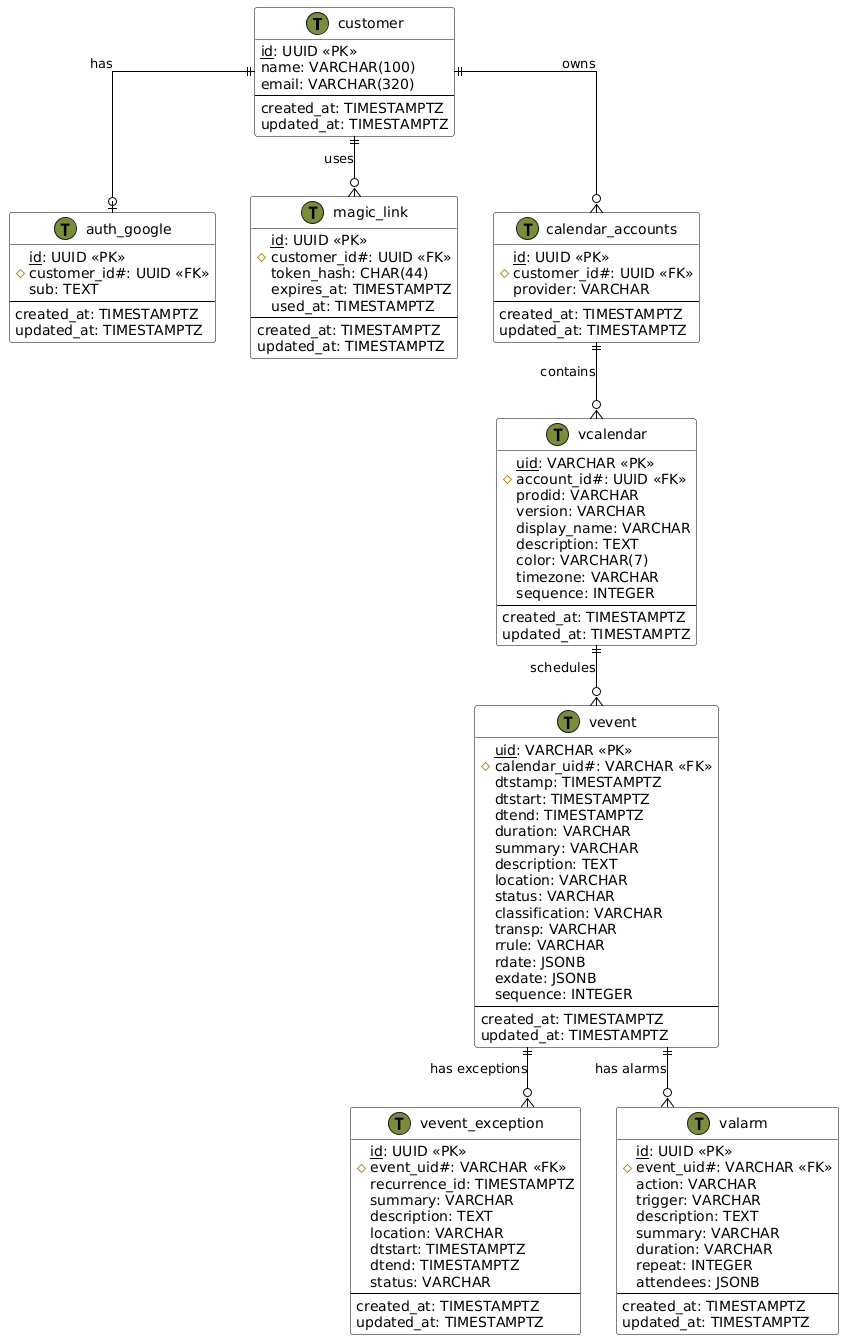
\includegraphics[width=0.9\textwidth]{images/docs/diagrams/er/database/Database Design.png}
    \caption{Entity-Relationship Diagram}
    \label{fig:er-diagram}
\end{figure}

\begin{figure}[!h]
    \centering
    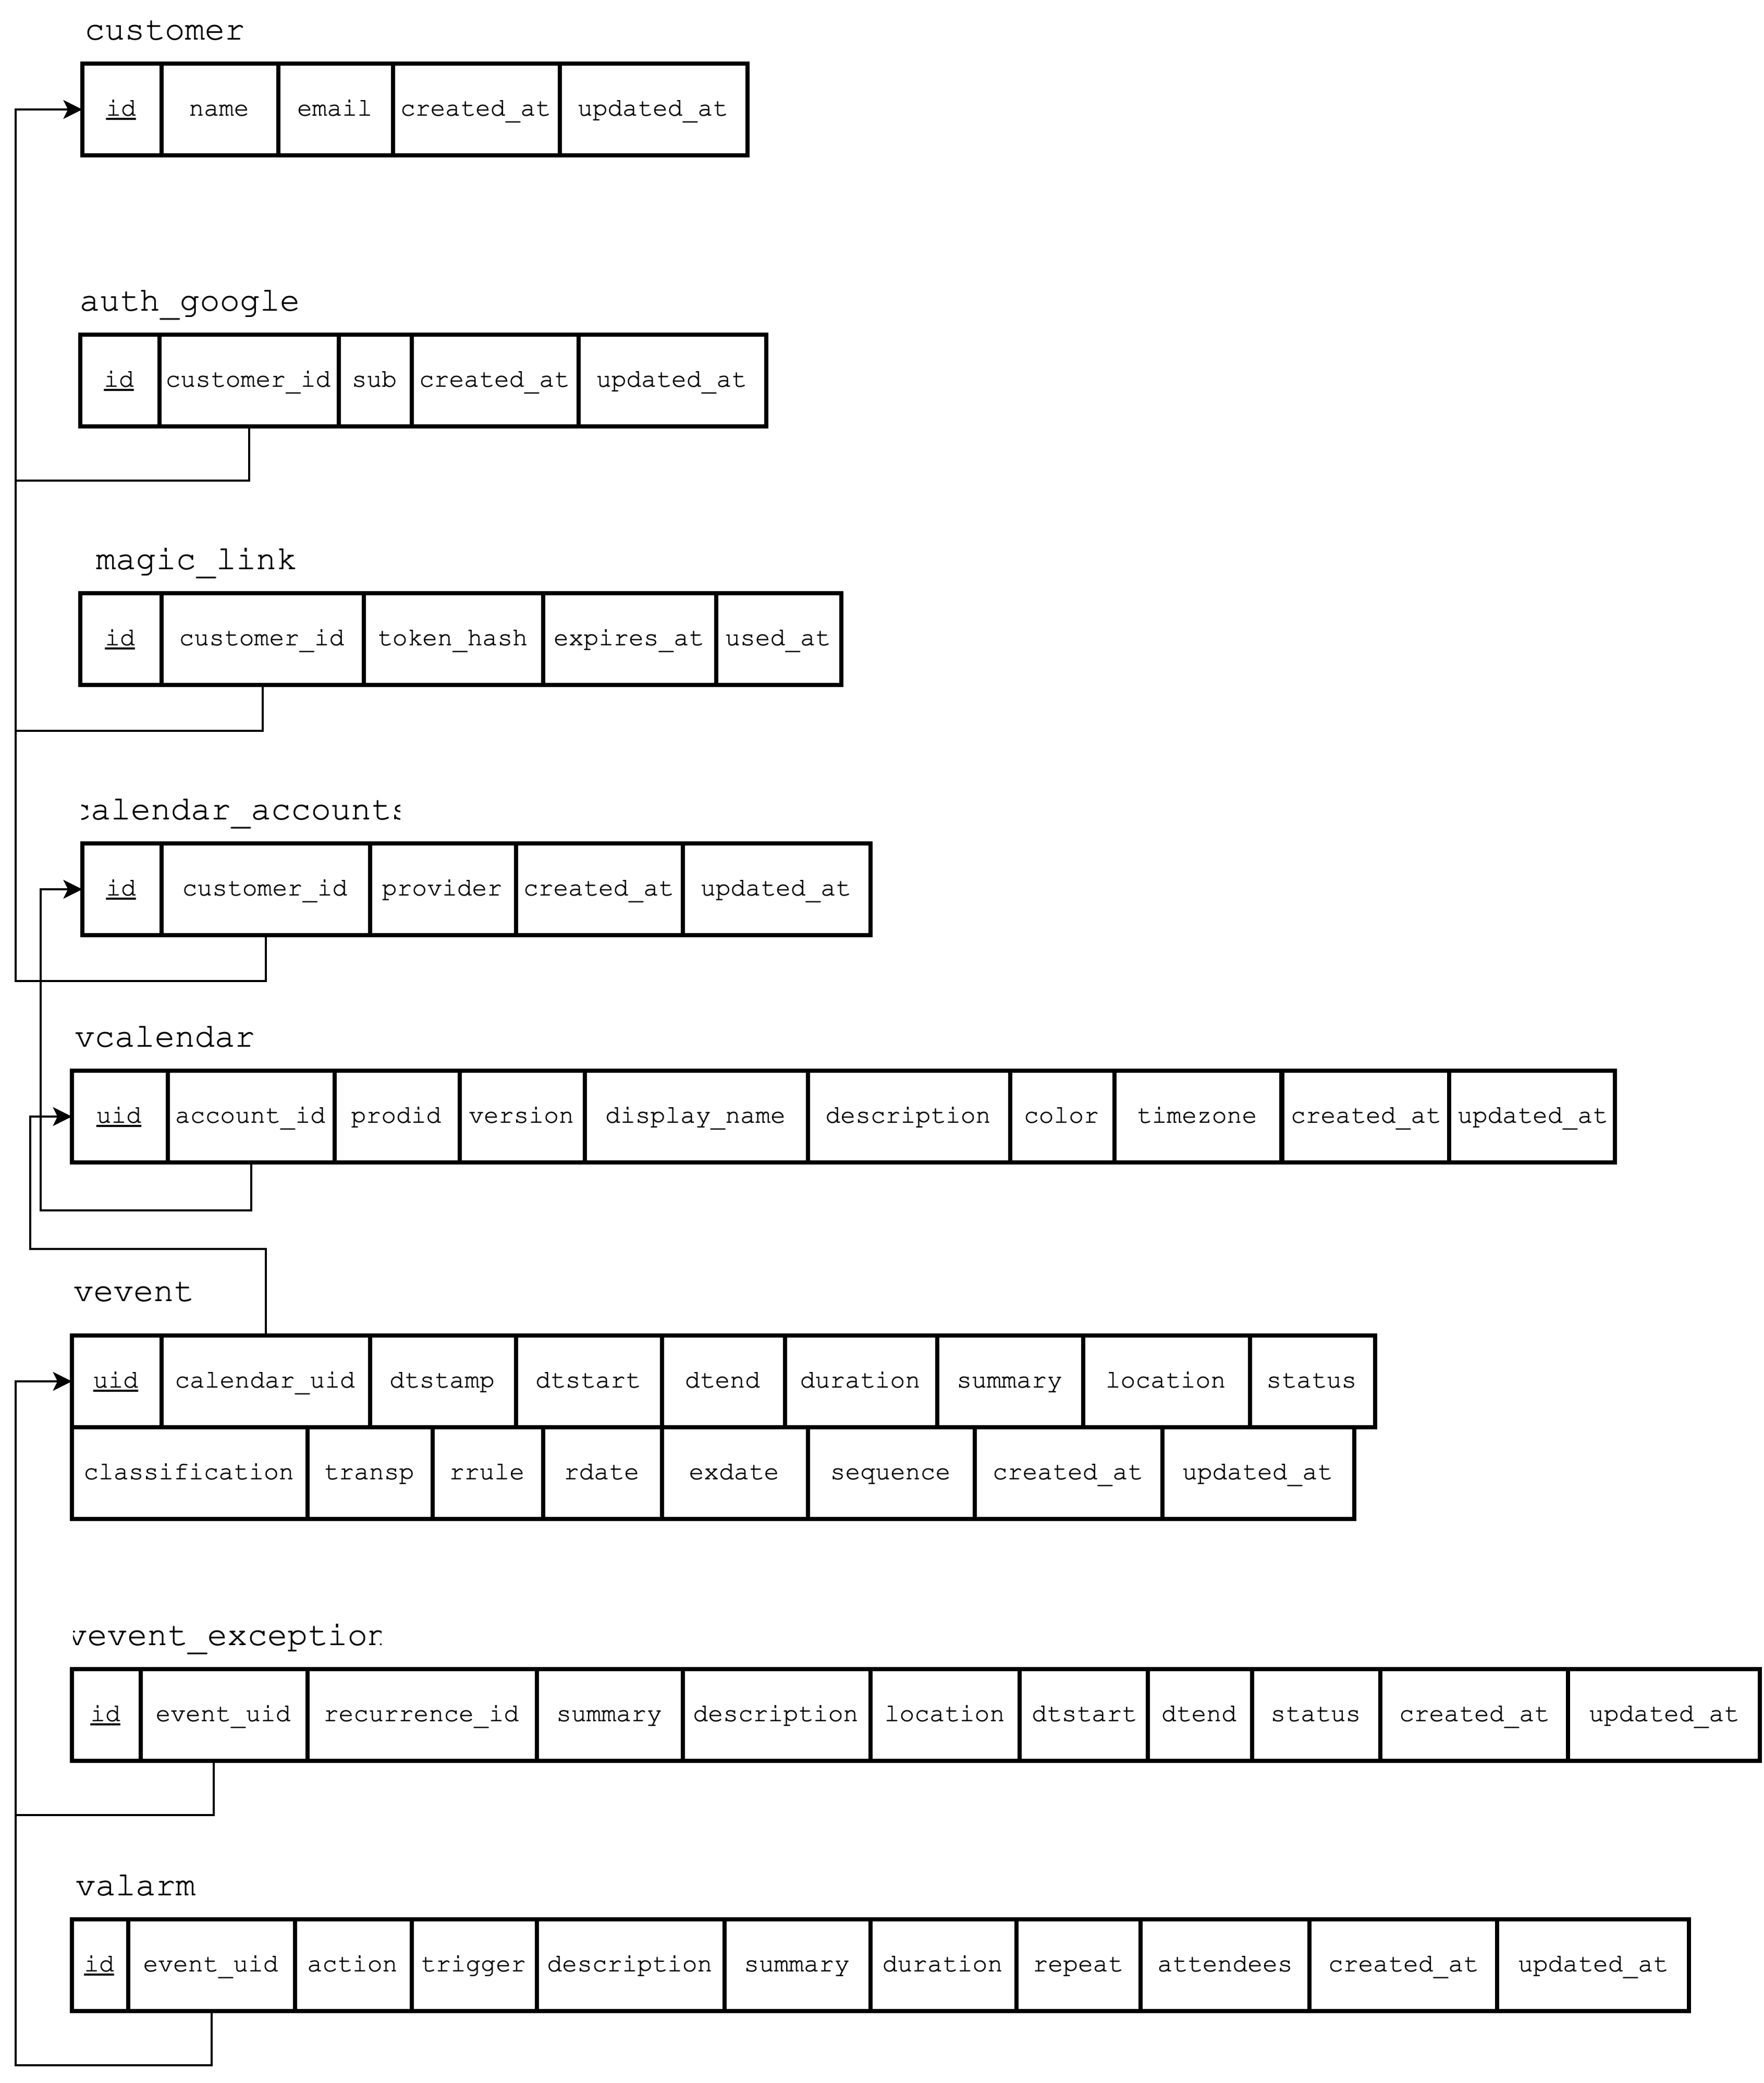
\includegraphics[width=\textwidth]{images/database-schema.png}
    \caption{Relational Schema}
    \label{fig:relational-schema}
\end{figure}

% ==========

\section{User Interface Prototype}

The user interface design of Jadwal plays a crucial role in delivering an intuitive and efficient calendar management experience. This section presents a comprehensive walkthrough of the application's key screens, from initial user onboarding to daily calendar interactions. The prototype demonstrates how Jadwal's core features—including authentication, calendar viewing, event management, and settings configuration—are implemented in a user-friendly manner that adheres to iOS design principles. Each screen has been carefully designed to balance functionality with simplicity, ensuring users can easily navigate and utilize all of Jadwal's features.

\vskip 2cm

\begin{figure}[!h]
    \begin{minipage}{0.3\textwidth}
        \centering
        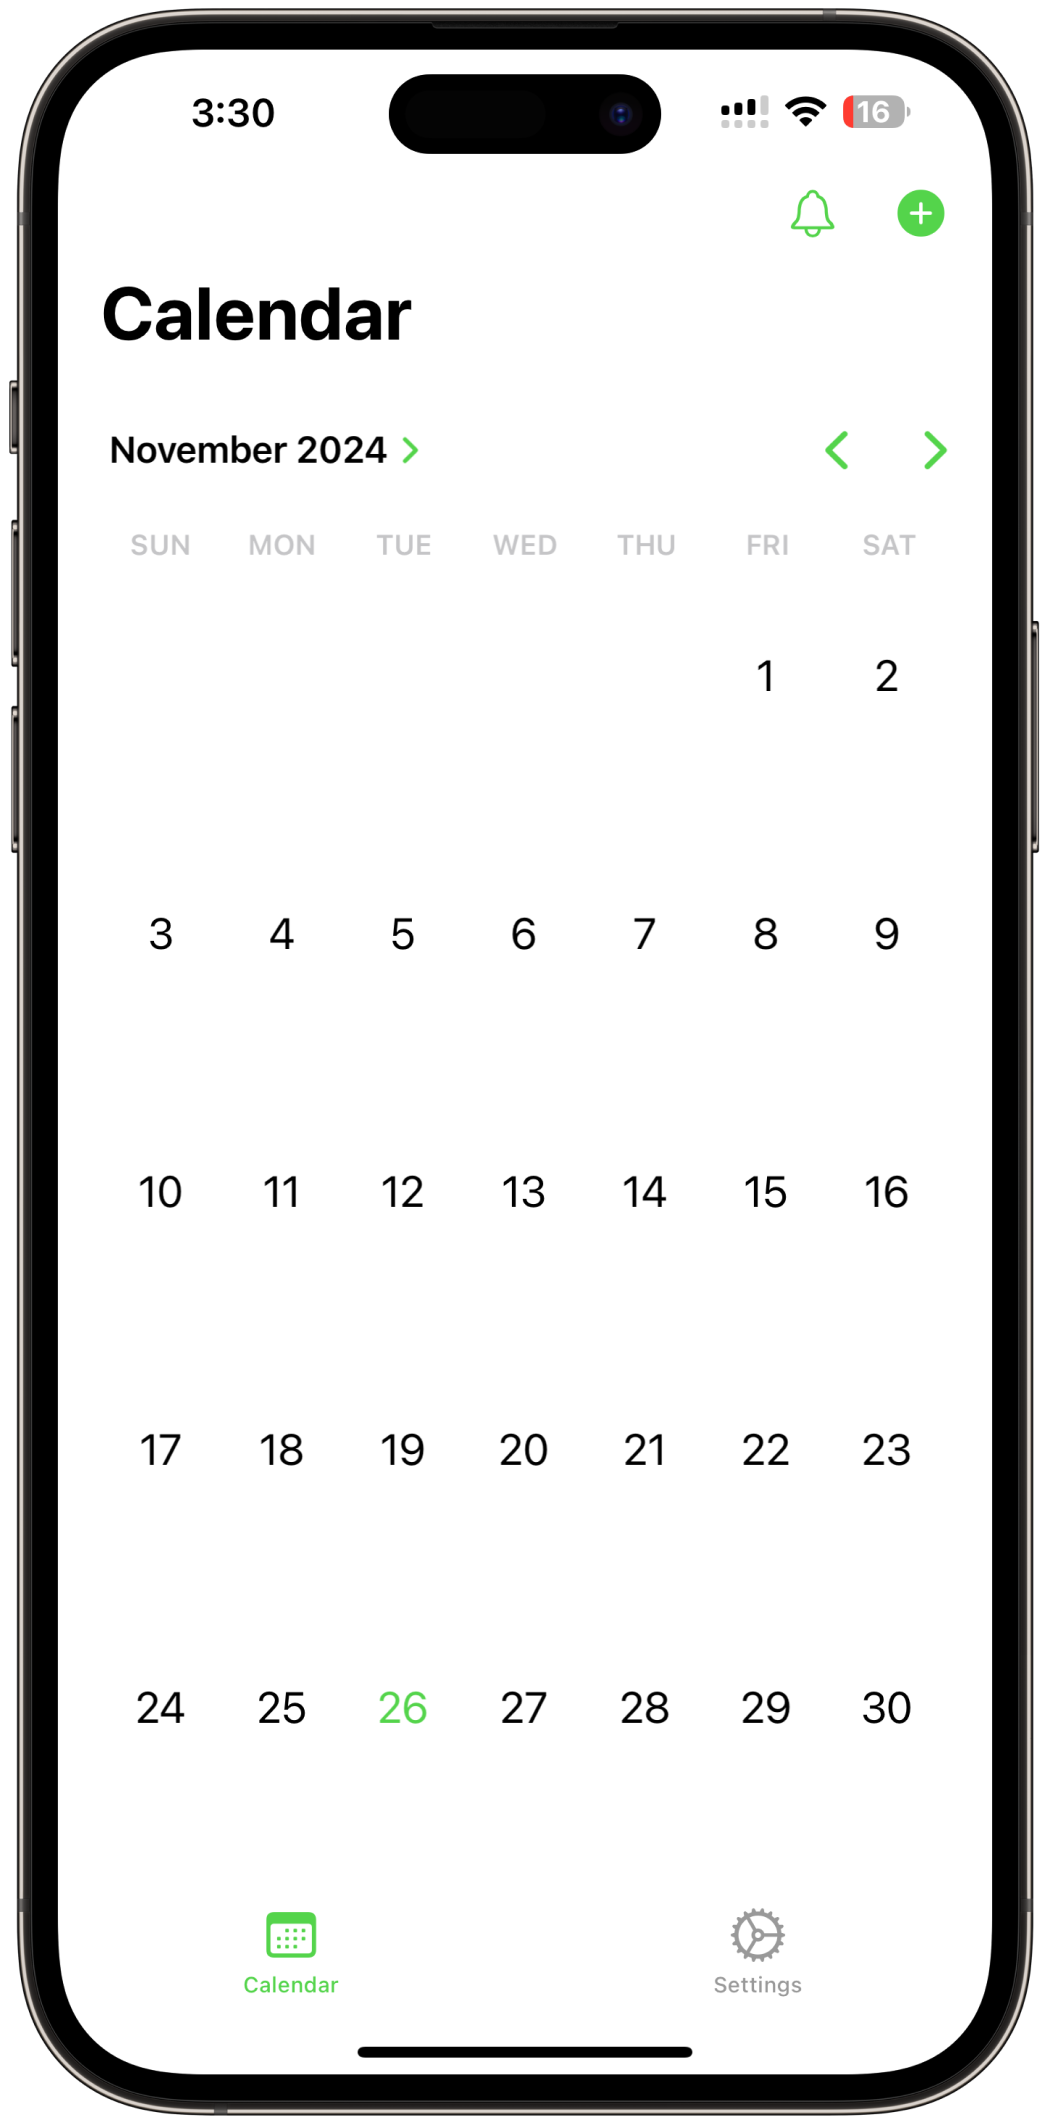
\includegraphics[width=\textwidth]{images/screen1.png}
        \caption{UI Screen 1: Onboarding View}
        \label{fig:ui-screen-1}
    \end{minipage}
    \hfill
    \begin{minipage}{0.65\textwidth}
        In Figure~\ref{fig:ui-screen-1}, the screen shows the user the steps he needs to take in the future so he knows what he is going to do. It also has two way of authenticating, Google and Email (Magic Link).
    \end{minipage}
\end{figure}

\begin{figure}[!h]
    \begin{minipage}{0.65\textwidth}
        In Figure~\ref{fig:ui-screen-2}, the screen is showing the continue with email screen which allows a user to enter their email, click "Continue", and receive an email if all is good.
    \end{minipage}
    \hfill
    \begin{minipage}{0.3\textwidth}
        \centering
        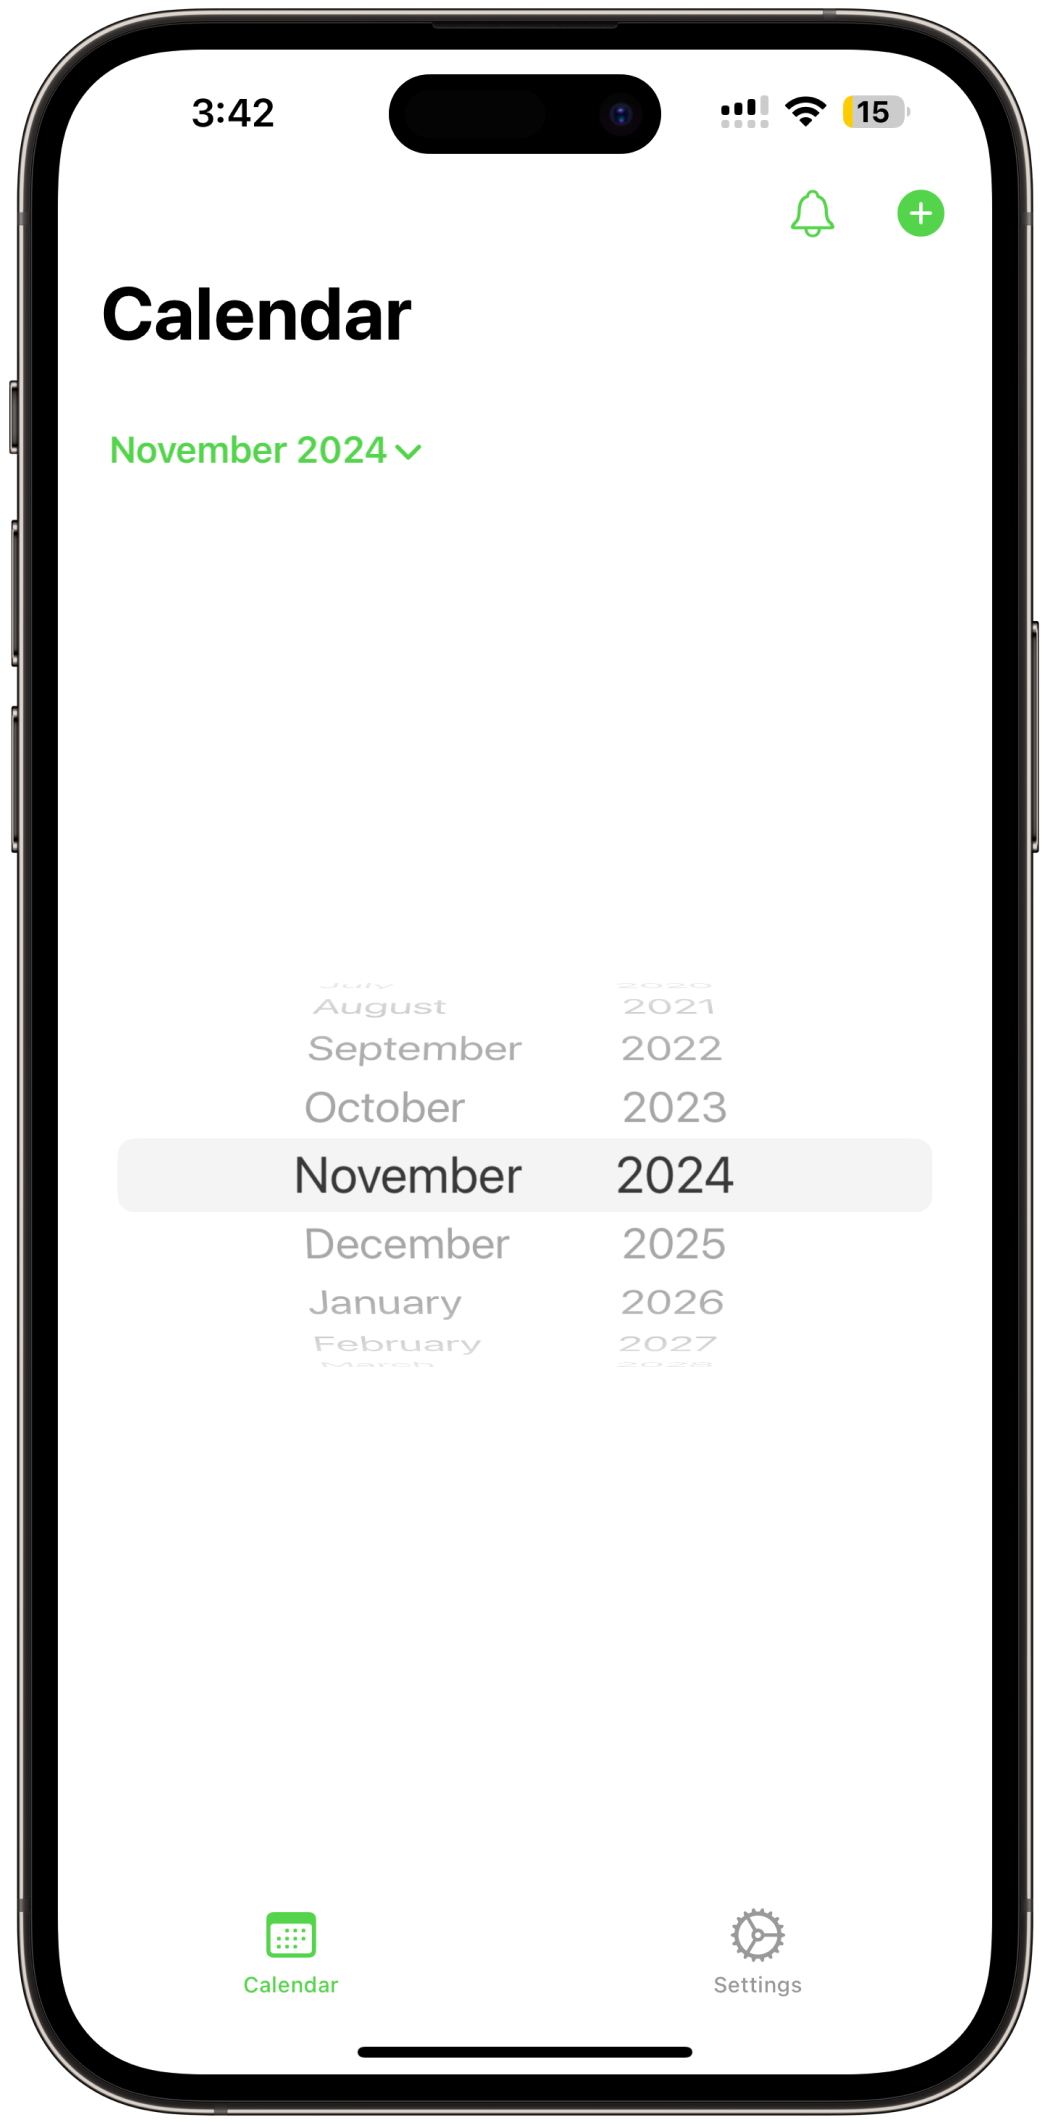
\includegraphics[width=\textwidth]{images/screen2.png}
        \caption{UI Screen 2: Continue with Email View}
        \label{fig:ui-screen-2}
    \end{minipage}
\end{figure}

\begin{figure}[!h]
    \begin{minipage}{0.3\textwidth}
        \centering
        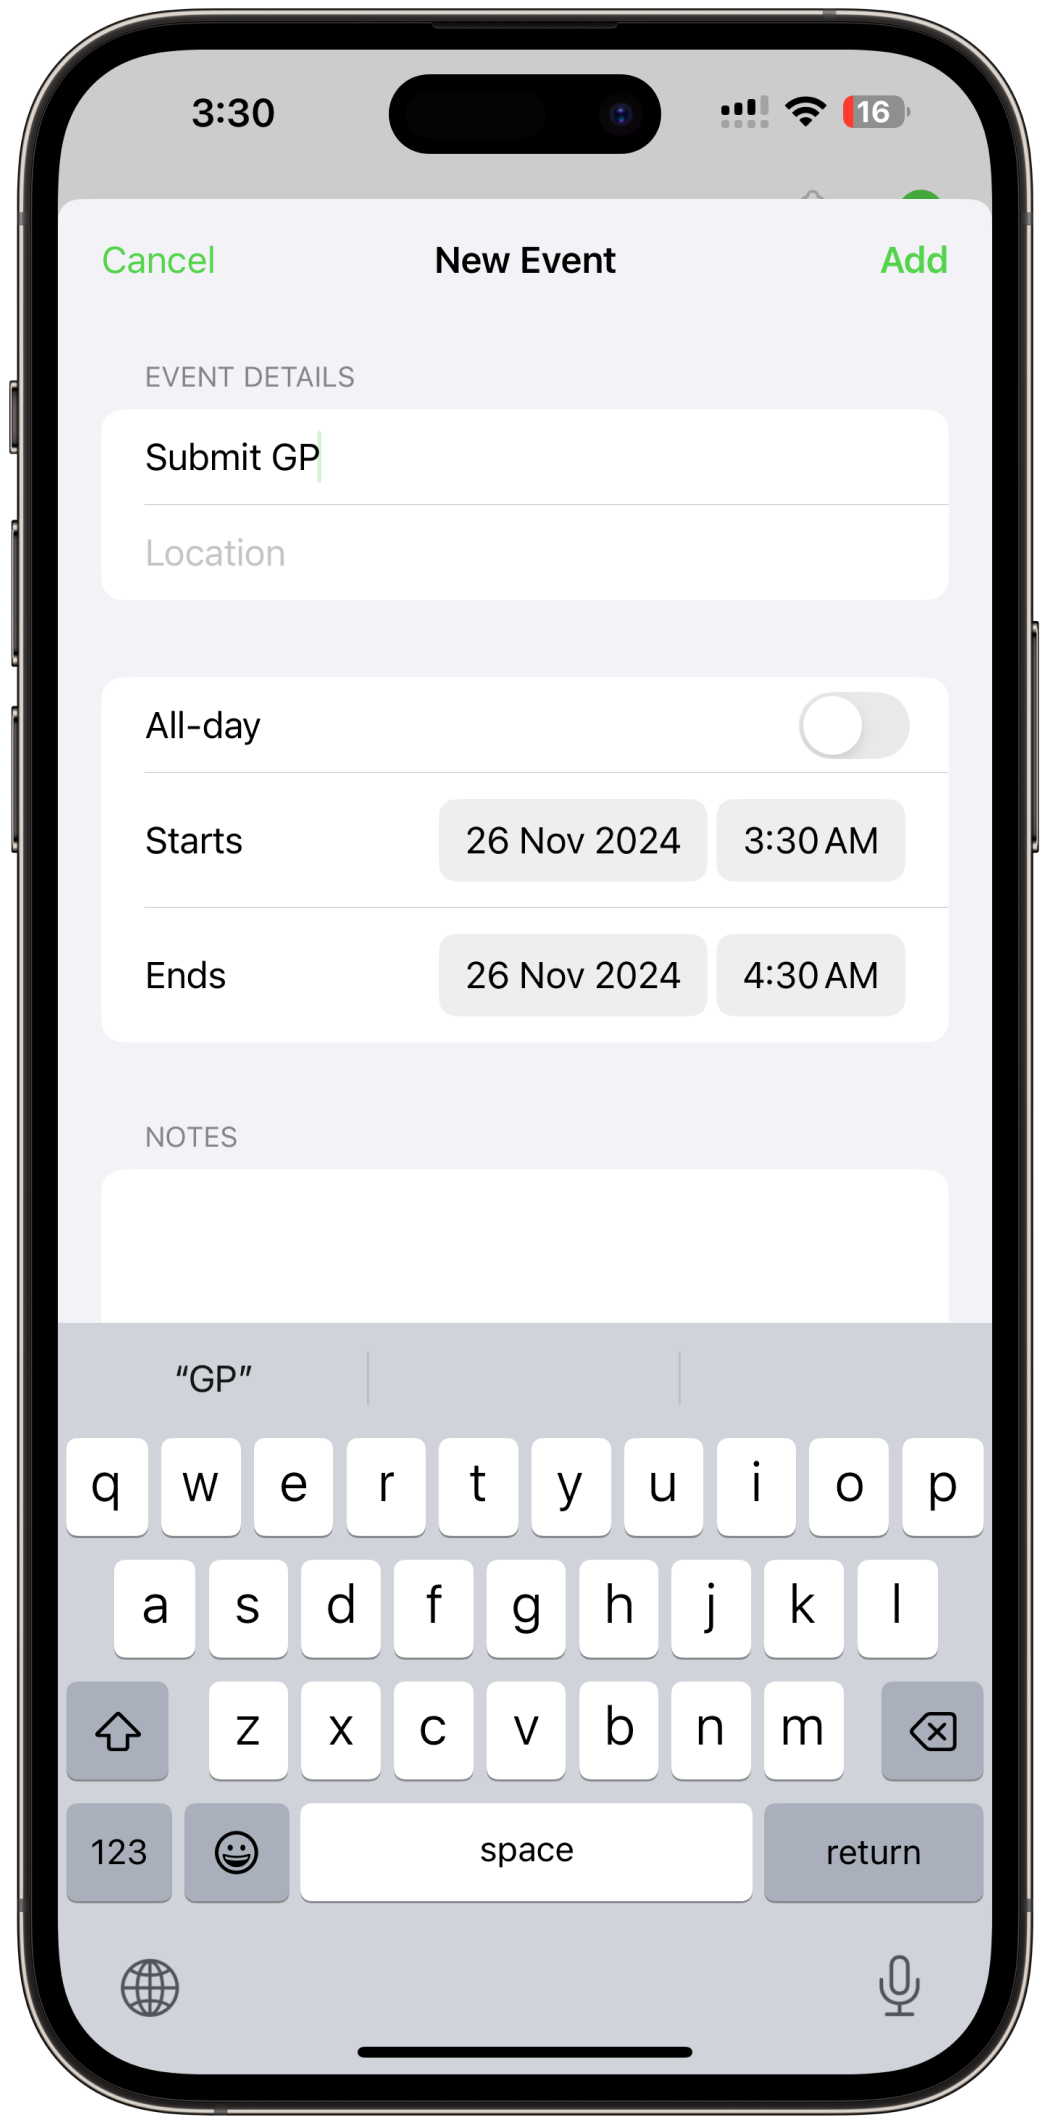
\includegraphics[width=\textwidth]{images/screen3.png}
        \caption{UI Screen 3: Check Your Email View}
        \label{fig:ui-screen-3}
    \end{minipage}
    \hfill
    \begin{minipage}{0.65\textwidth}
        In Figure~\ref{fig:ui-screen-3}, the screen that tells the user to check their email for the magic link is shown. They can also click "Resend Email" to get another copy if the first one wasn't received. If they received it, they can click the link inside it and it will redirect back to the app and the app will be able to read the url and its contents which has a token which the app uses to finish the authentication process. Once the authentication process is done, the user is moved to the screen shown in Figure~\ref{fig:ui-screen-4}
    \end{minipage}
\end{figure}

\begin{figure}[!h]
    \begin{minipage}{0.65\textwidth}
        In Figure~\ref{fig:ui-screen-4}, the calendar view represents the user's schedule. It shows upcoming events, past events, and current events. It also has two buttons at the top, notifications and add event buttons. Users can swipe left and right to navigate months. The current day is colored in green.
    \end{minipage}
    \hfill
    \begin{minipage}{0.3\textwidth}
        \centering
        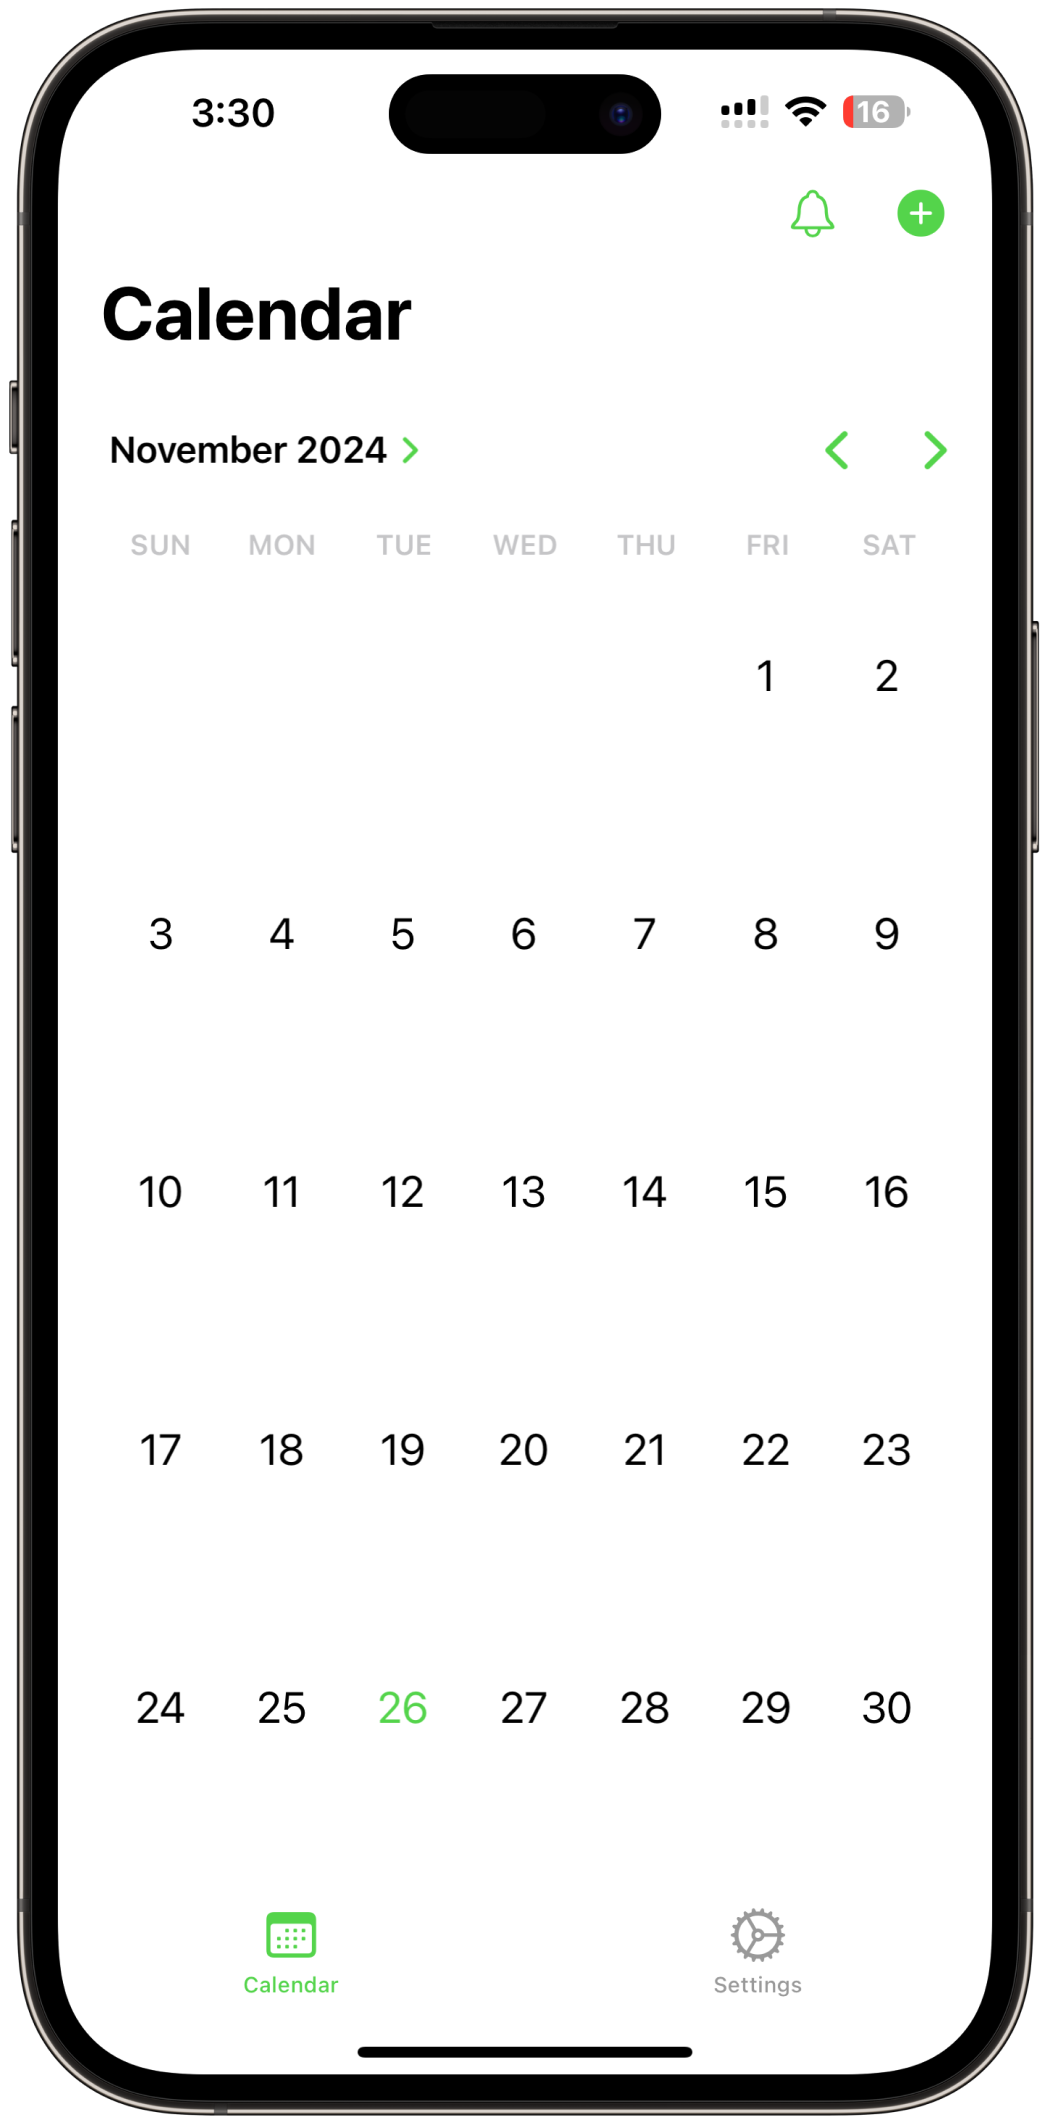
\includegraphics[width=\textwidth]{images/screen4.png}
        \caption{UI Screen 4: Calendar View}
        \label{fig:ui-screen-4}
    \end{minipage}
\end{figure}

\begin{figure}[!h]
    \begin{minipage}{0.3\textwidth}
        \centering
        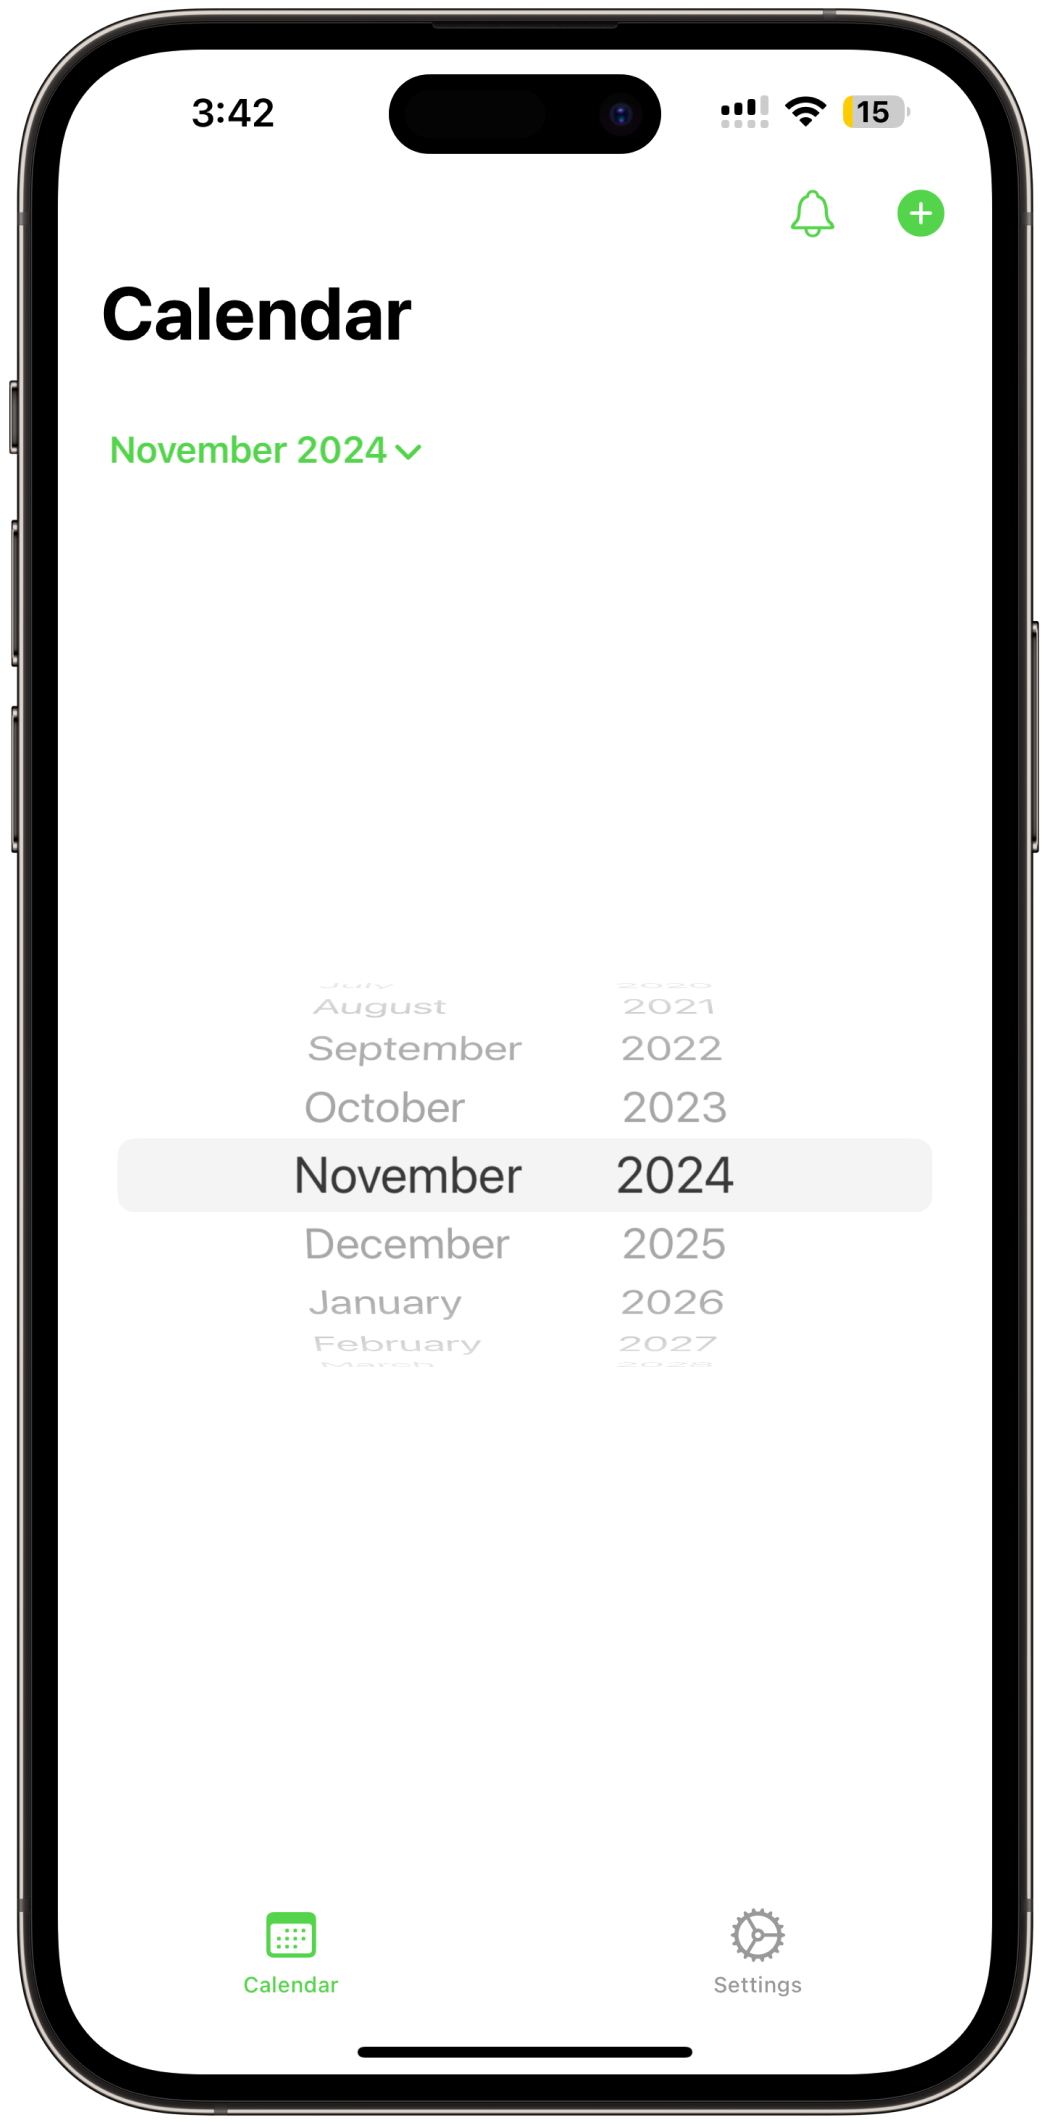
\includegraphics[width=\textwidth]{images/screen5.png}
        \caption{UI Screen 5: Month \& Year Selector}
        \label{fig:ui-screen-5}
    \end{minipage}
    \hfill
    \begin{minipage}{0.65\textwidth}
        In Figure~\ref{fig:ui-screen-5}, users can click on the text that shows the currently selected month, in this case ``November 2024'' and get a selector wheel that allows them to choose a month and a year to navigate to.
    \end{minipage}
\end{figure}

\begin{figure}[!h]
    \begin{minipage}{0.65\textwidth}
        In Figure~\ref{fig:ui-screen-6}, the screen is showing the add event sheet in its default state. It is shown when you click the "add event" button in Figure~\ref{fig:ui-screen-4}.
    \end{minipage}
    \hfill
    \begin{minipage}{0.3\textwidth}
        \centering
        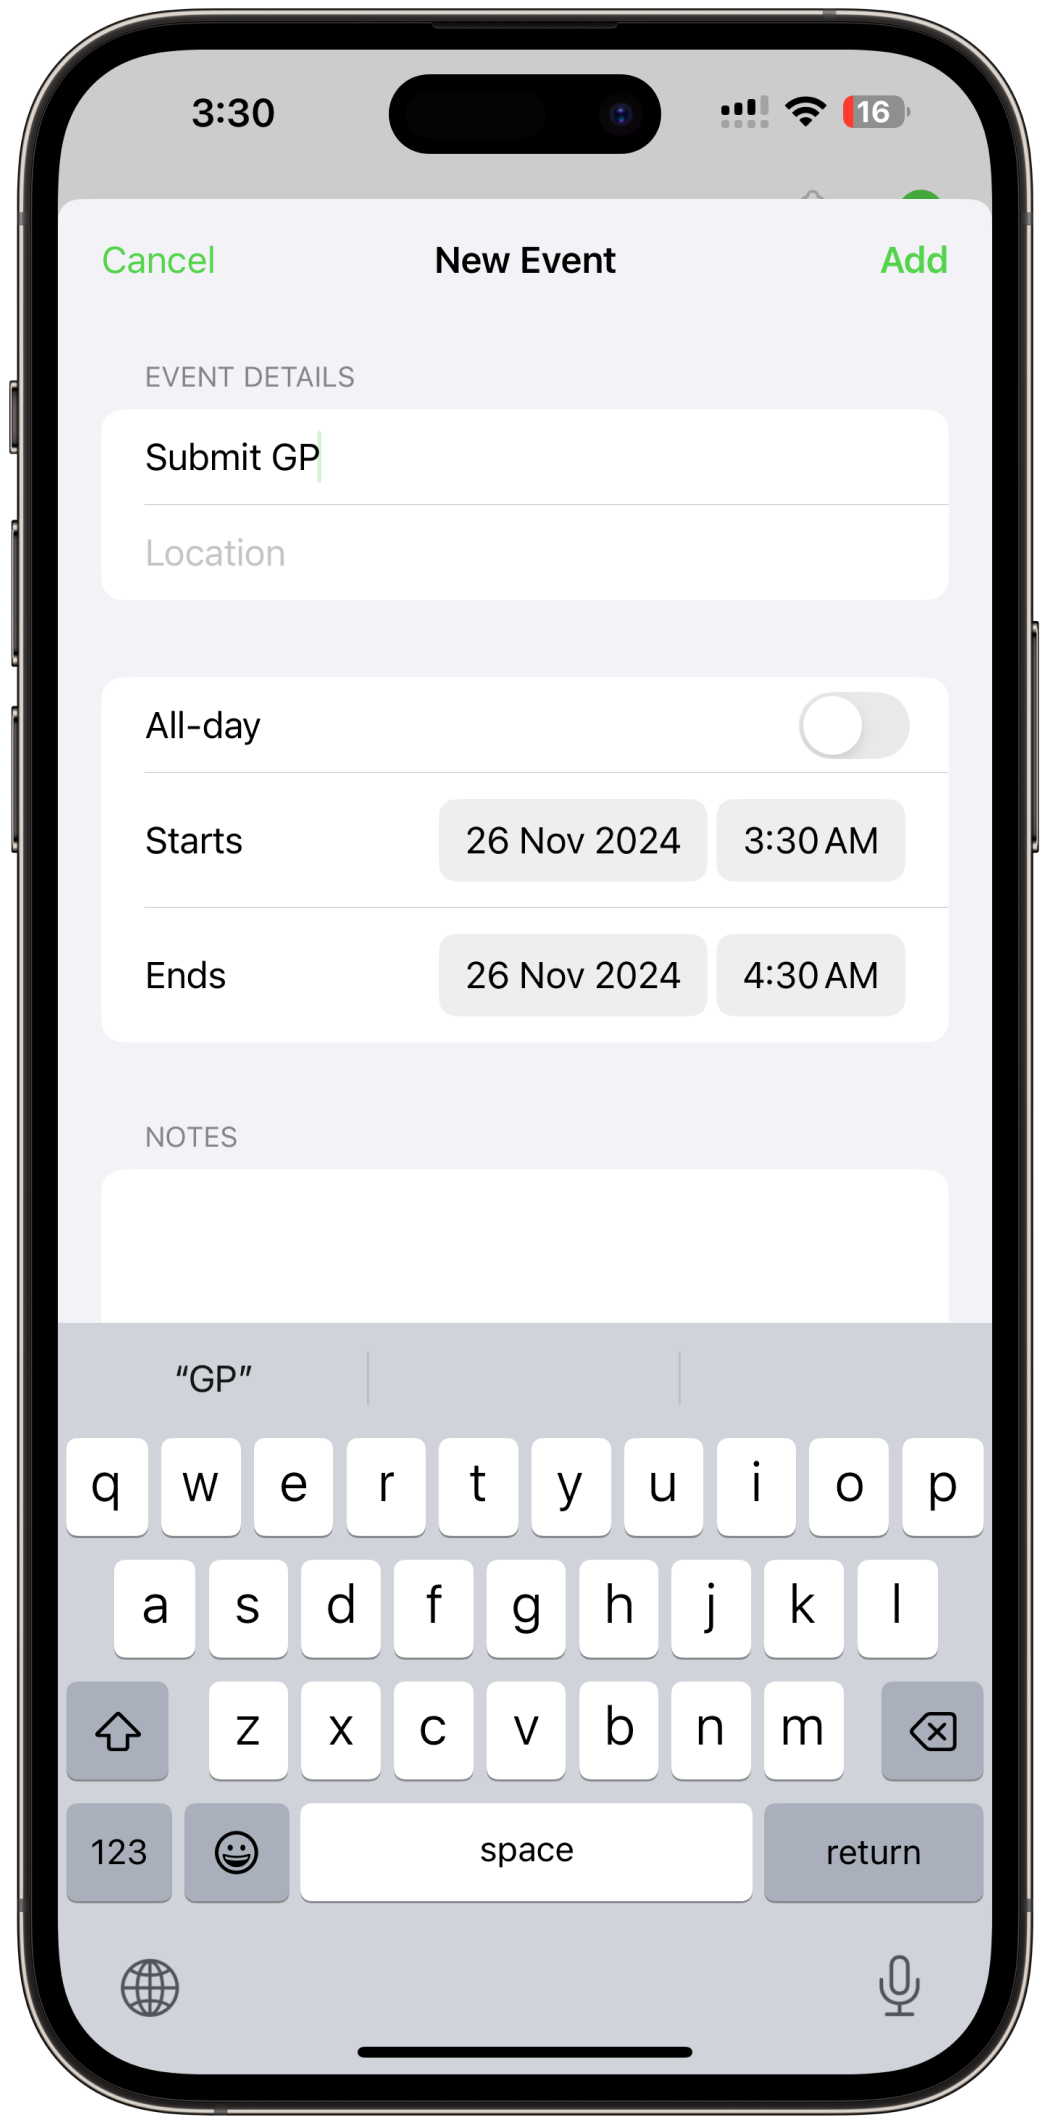
\includegraphics[width=\textwidth]{images/screen6.png}
        \caption{UI Screen 6: Add Event View - Default}
        \label{fig:ui-screen-6}
    \end{minipage}
\end{figure}

\begin{figure}[!h]
    \begin{minipage}{0.3\textwidth}
        \centering
        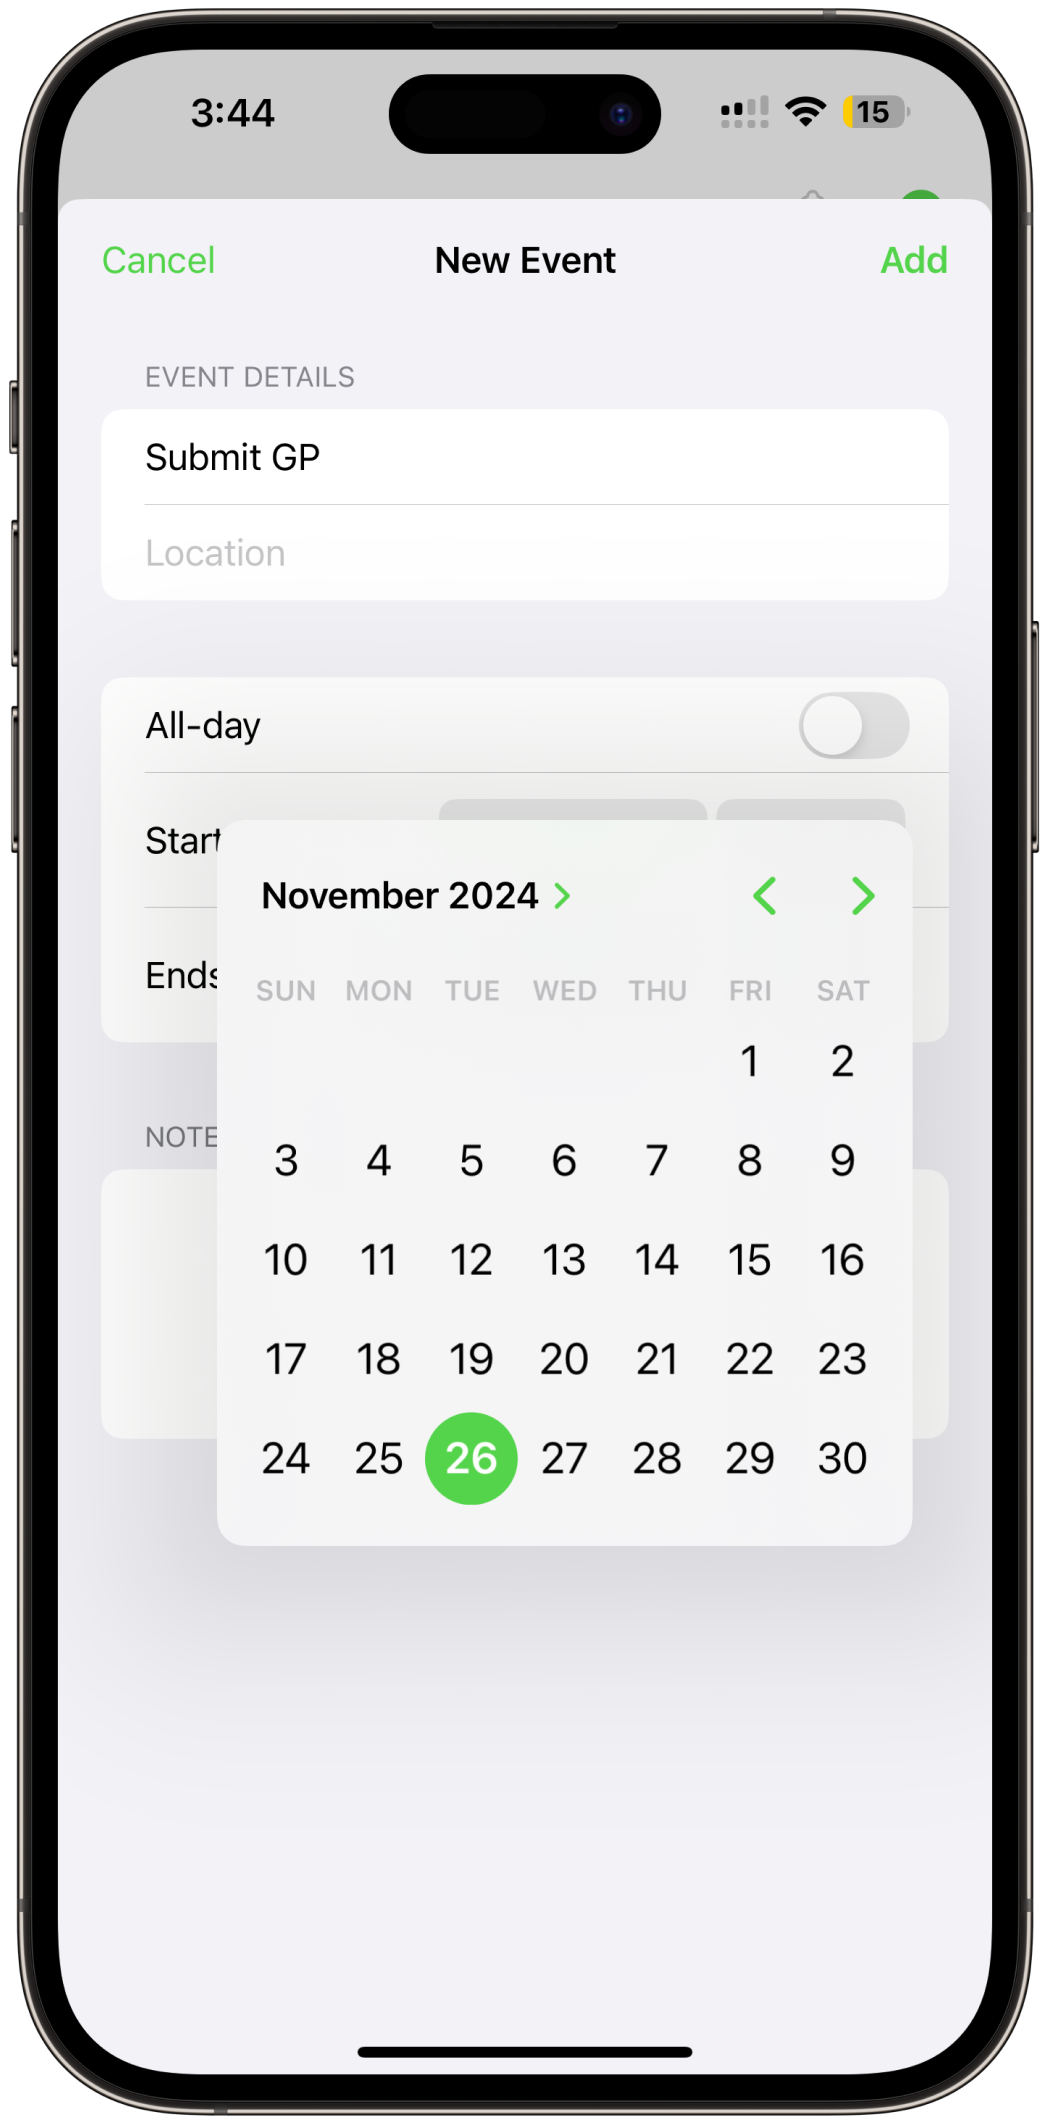
\includegraphics[width=\textwidth]{images/screen7.png}
        \caption{UI Screen 7: Add Event View - Date Picker}
        \label{fig:ui-screen-7}
    \end{minipage}
    \hfill
    \begin{minipage}{0.65\textwidth}
        In Figure~\ref{fig:ui-screen-7}, the screen is showing the add event sheet in its date picker chosen state. You can choose a date and scroll between months and years if you want.
    \end{minipage}
\end{figure}

\begin{figure}[!h]
    \begin{minipage}{0.65\textwidth}
        In Figure~\ref{fig:ui-screen-8}, the screen is showing the add event sheet in its time picker chosen state. You can choose a time and scroll between hours and minutes if you want.
    \end{minipage}
    \hfill
    \begin{minipage}{0.3\textwidth}
        \centering
        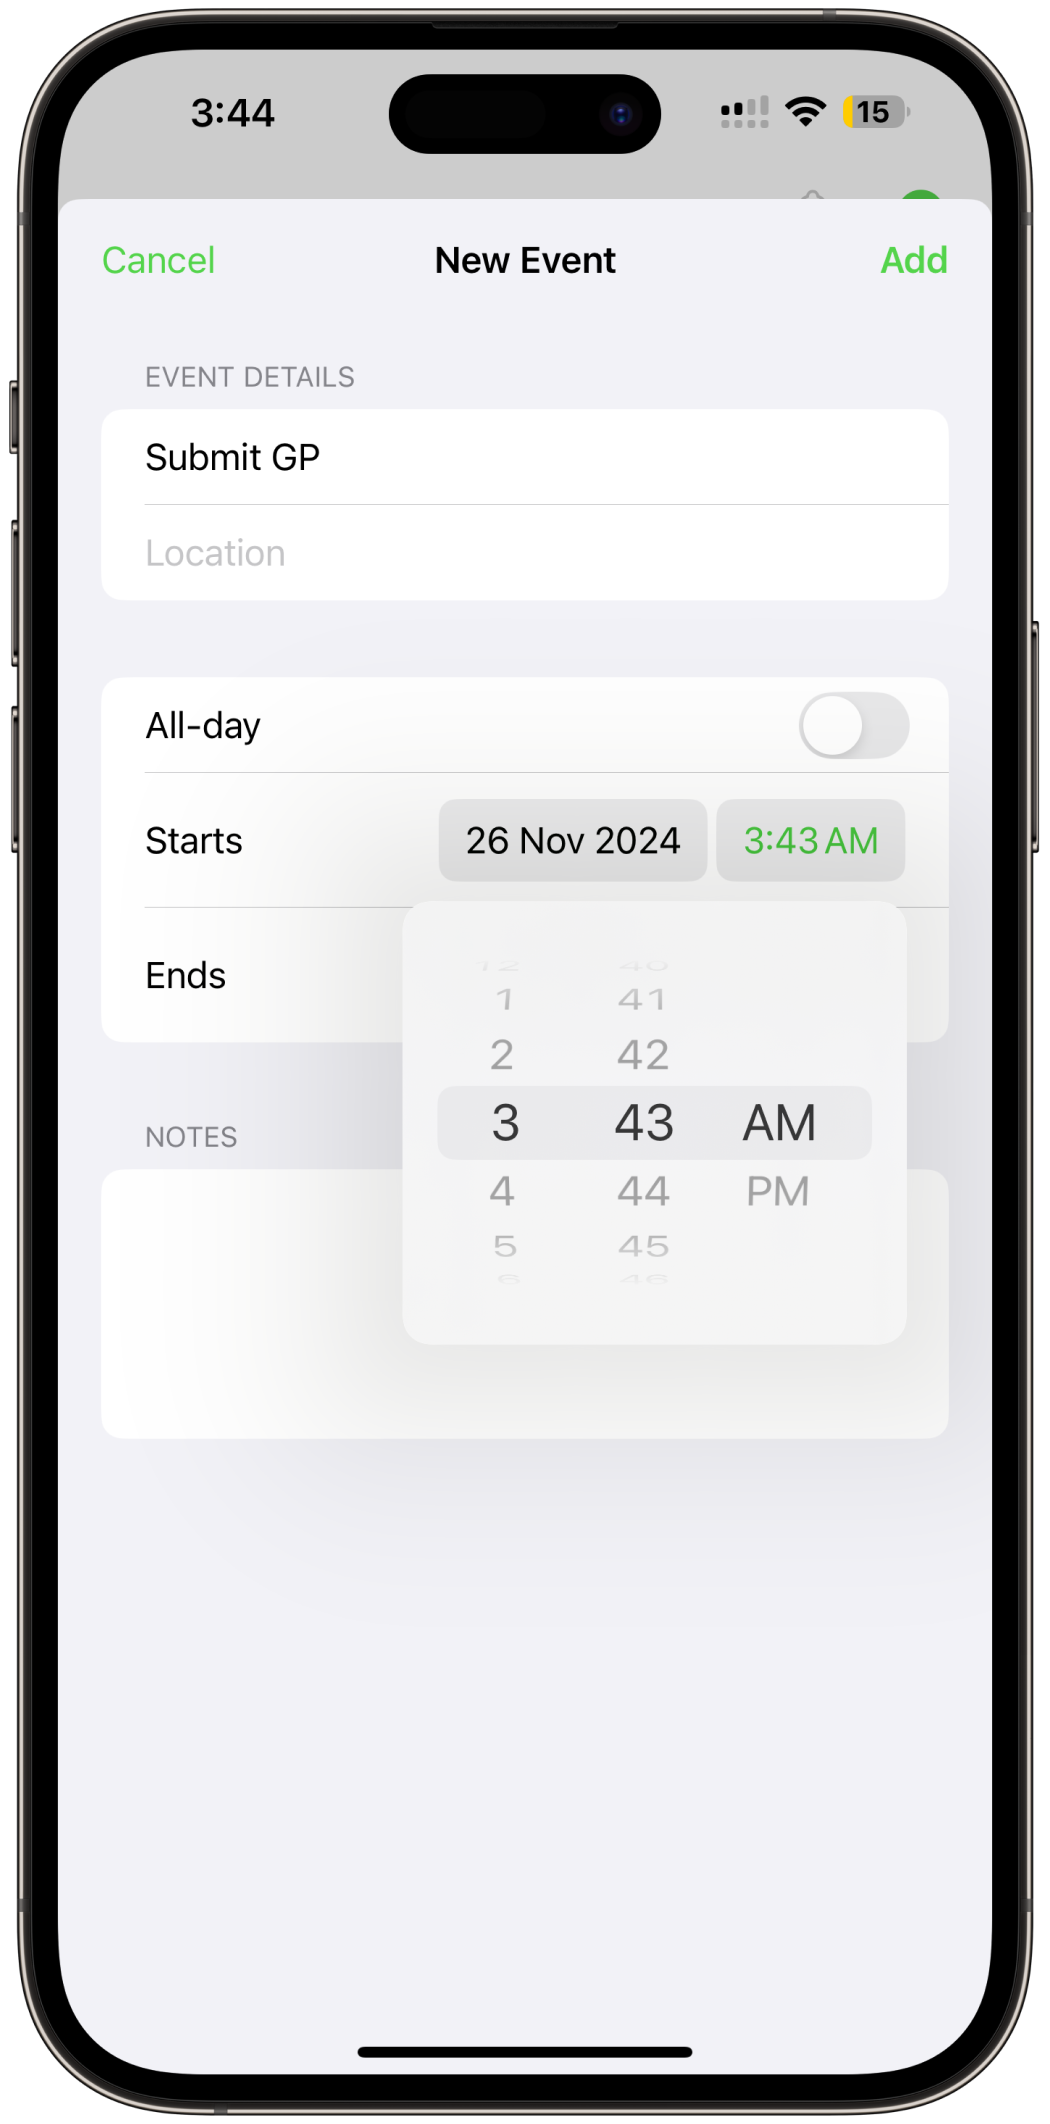
\includegraphics[width=\textwidth]{images/screen8.png}
        \caption{UI Screen 8: Add Event View - Time Picker}
        \label{fig:ui-screen-8}
    \end{minipage}
\end{figure}

\begin{figure}[!h]
    \begin{minipage}{0.3\textwidth}
        \centering
        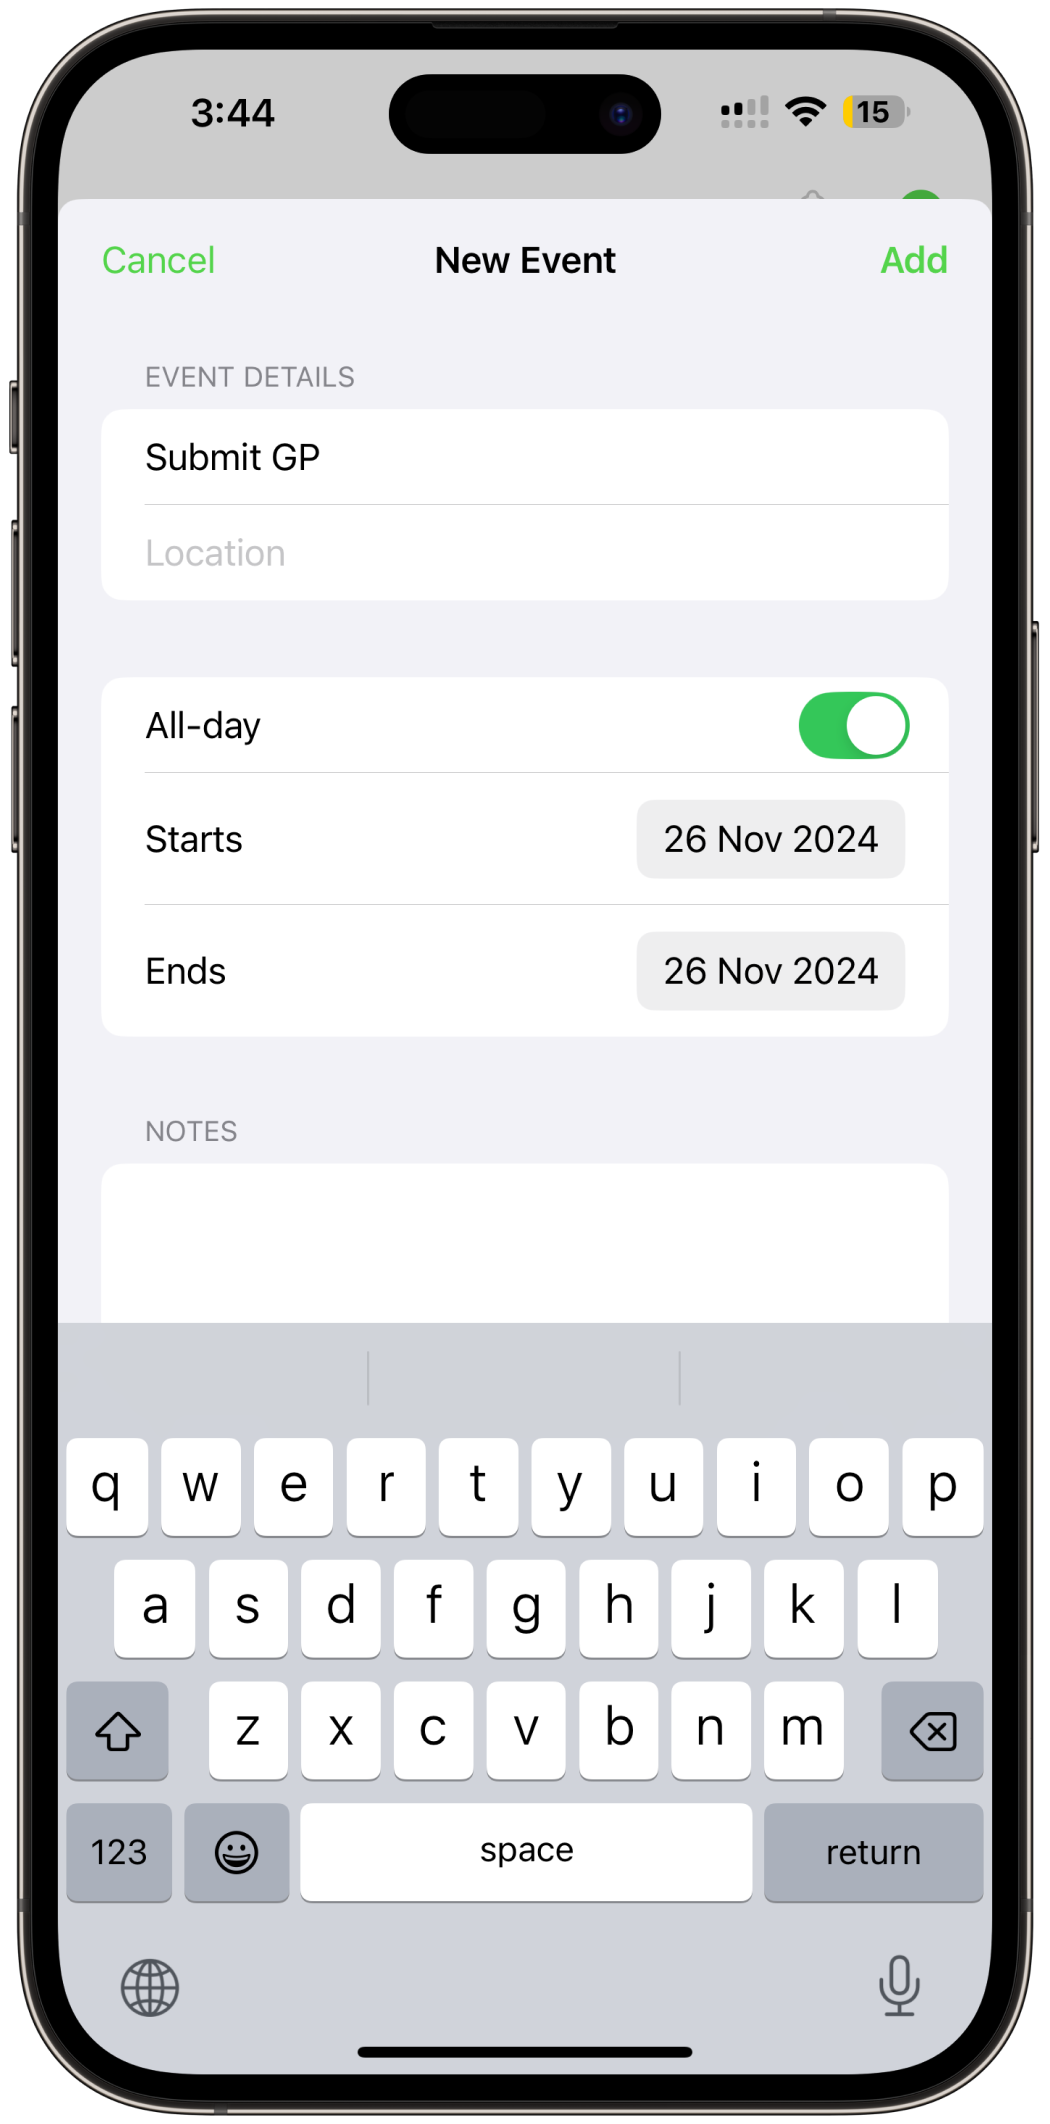
\includegraphics[width=\textwidth]{images/screen9.png}
        \caption{UI Screen 9: Add Event View - All Day}
        \label{fig:ui-screen-9}
    \end{minipage}
    \hfill
    \begin{minipage}{0.65\textwidth}
        In Figure~\ref{fig:ui-screen-9}, the screen is showing the add event sheet in its all day state. That means you only choose the dates, no need for the times.
    \end{minipage}
\end{figure}

\clearpage

\begin{figure}[!h]
    \begin{minipage}{0.65\textwidth}
        In Figure~\ref{fig:ui-screen-10}, the settings page is shown. This page has the user details, specifically email, and name. Also the "Connect WhatsApp" button is shown along with the "Connect CalDAV" button. Those two buttons do as they say and allow users to have data sources for the calendar connected. The last button shown is the logout button, and this button is in red to make the user alerted and not click it by mistake. Clicking it will log the user out and take them to the home screen.
    \end{minipage}
    \hfill
    \begin{minipage}{0.3\textwidth}
        \centering
        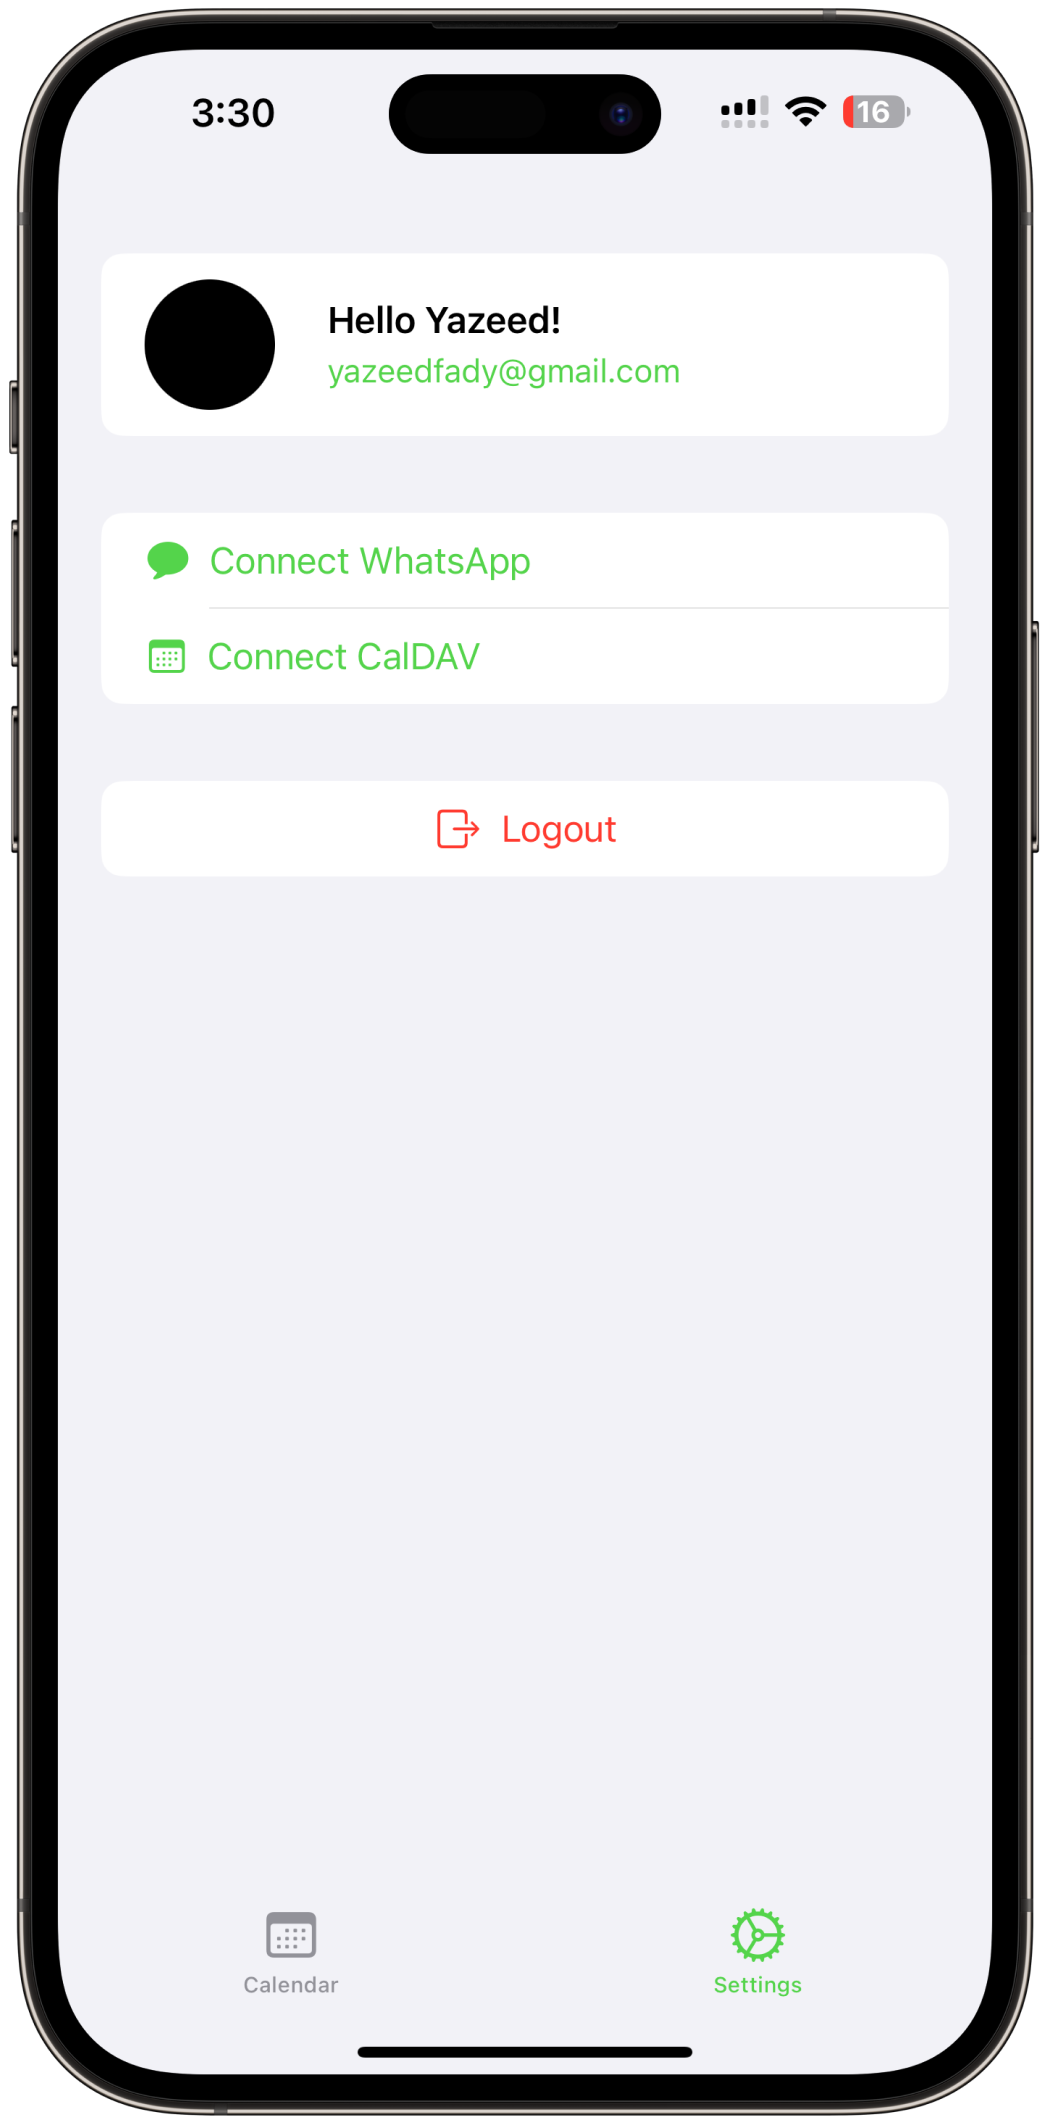
\includegraphics[width=\textwidth]{images/screen10.png}
        \caption{UI Screen 10: Settings View}
        \label{fig:ui-screen-10}
    \end{minipage}
\end{figure}

\vfill

\section{Conclusion}
Jadwal stands as a comprehensive and innovative solution for scheduling with great design. The use cases and database architecture are well described, which helps in creating the application systematically. The use cases clearly define how users interact with the system, covering all the features like Continue with email, Resolve conflicts, WhatsApp integration, scheduling prayer time, and many more. The database design is the backbone of Jadwal, which clearly shows how the system works and how the data is managed perfectly. In conclusion, Jadwal is well described, which makes it easy to understand how everything is working and would be easy to track everything that is happening in the backend.

\vfill

% ==========

\cleardoublepage
